\section{Development timeline}

This section will follow the conceptualization and implementation of
the game ''People With Guns''. The back end and mechanics of the game will be
analyzed and presented in their evolution, also briefly describing aspects of
the front end. \newline

In this chapter, we will see the steps taken until the idea for the game has
been crystalized. Then, we will follow the steps of development and field
testing of the server and client, chronologically.


\subsection{The exploration phase}

The development of the app has started on the 14th of January 2013.
The evolutionary steps and intermediary and final concepts are presented here.\newline

\subsubsection{Creating the game concept}

The project had started as a proposal to add a multiplayer feature to a tour
app. Simply adding the functionality to see all the others within the group on
the map was not sufficient - it would just help if someone got lost or went
astray. Otherwise, it was concluded that the user experience would not be
improved in any significant way. Then came the idea of adding small games,
hidden caches or quests and so on. The best idea that still had the tour app as
a main platform was to add detours from the main track as bonuses. On those
detours, the people would have to solve various riddles and small puzzles to get
points and find out about hidden historical spots or interesting facs about the
places they are visiting. \newline

At this point, the following addon to the main app was contoured: the
players would have a main tour path and, as they passed by certain waypoints,
would be offered to go through a bonus/extra track within the area that they are
visiting. If enough of them would agree to do this(by an in-app vote, for
example), they would be presented with a new set of waypoints. These waypoints
would belong to a number of categories: normal waypoints, waypoints where they
would have to split, waypoints where they would have to be together and
waypoints where the whole group would have to wait within a virtual circle,
while one delegate(through vote) would find an item or solve a riddle -
of course, with the help of the entire group.\newline

Another scenario has been proposed, during the research: In the case of the
group waiting and one member being delegated to solve a riddle or find an item,
a means of cooperation can be brought up: When the team votes and chooses the
delegate, his screen turns black(no map) and the rest of the team can see
the goal on their phones. Through messages or in-app voice communication,
they would help the delegate navigate to the goal. Then, once the goal has been
found or reached, the virtual circle would disappear and the whole team would be
free to move. If anyone would exit the circle at some point, they would receive
penalties and eventually get disconnected from the game.\newline

Gradually, the ideas for multiplayer features went astray from the tour app,
towards multiplayer GPS-based games. The idea of GPS-based puzzle / adventure
games was explored ARIS was encountered - a platform for creating such games.
Then Tourality was discovered, and WarFinger GPS, which have been the main
sources of inspiration for the 'War Game' and a few other games that didn't make
it in the main concept, but are to be developed within the game as future
work.\newline

There has been a point when all the GPS-based mobile games that could be
found were studied and where possible, played. Then they were evaluated for
advantages, disadvantages and gameplay. At this point, the goals for the game to
be developed were already in mind: It should move the players to an outdoor
environment and have them walk and run as the main activity, while using the
game itself for an improved experience. Hide and seek and Tag were considered as
a model of entertaining game to be played by a group. The games found and
already enumerated can be considered to have one of two major disadvantages:

\begin{enumerate}
  \item Do not engage the users enough: Games such as Parallel Mafia, SCVNGR or
  Please Stay Calm do not motivate the player to move around much. They also
  offer a very dim user experience in areas with few or no players.
  \item Engaged the users too much: Mobile users, even hardcore gamers, do not
  spend too much time playing on the phone. Rather, they would play on consoles
  or computers, for better immersion. No matter how good the game is, it is
  still displayed on a small phone screen(tablets are not considered in this
  paper). Games such as Ingress and Shadow Cities offer a better and more
  immersive story, but are still demanding of the player and request the full
  focus of the phone owner. This can be considered as a major downside, as at
  least some people(the author included), do not want to be engaged for
  prolonged amounts of time, nor to deviate from their usual trips through
  the city for the sake of a game, nor will they spare the time and will to play
  such a demanding game while on the go.  
  \item Do not motivate the players to move enough - Only Tourality does not
  possess this downside, as it its various game modes are specifically designed
  for running.
  \item Are location-dependent - All adventure / puzzle games such as those
  developed with ARIS, most MMOs such as Parallel Mafia do require the player to
  be in certain places in order to progress through the game. This means that
  the player is put in one of two situations : he 1. has to get out of
  his way in order to make any progress within the game, or 2. has to travel
  to remote locations in order to play the game in the first place. This might
  be interesting for some, but does not cover a broad spectrum of population. 
\end{enumerate}

The engagement problem can also be linked to a time problem. Games that are
highly engaging also require a lot of time to be played. The arugment that the
amount of time dedicated to the mobile game should be decided by the player and
not by the game has been used in the construction of the concept of the game
that was eventually developed. \newline

\subsubsection{The game concept}
The app developed is temporarily called ''People With Guns''. It is a GPS-based
Real Time Tactics game with Shooter elements, developed for Android. It can be
played by several people (The upper limit has not been established yet. Until
now, the highest number of players in the game has been six) that choose to join
one of the two opposing teams. The purpose of the game is to use 'weapons' and
'powerups' to defeat the opposing team. By 'defeat', we mean to use the
available tools provided by the game to reduce the virtual 'health' attribute of
all the opponents to zero.\newline

The current 'tools' are as follows :\newline

The weapons : 
\begin{enumerate}
  \item Pistol
  \item Rifle
  \item Sniper Rifle
  \item Knife   
\end{enumerate}

The 'powerups' :
\begin{enumerate}
  \item Invisiblity Cloak
  \item Shield
  \item Painkillers / Heal
\end{enumerate}

Each item used by a player has the following attributes : 
\begin{enumerate}
  \item Cooldown - The amount of time that has to pass until the weapon can be
  used again.
  \item Duration - The amount of time during which a powerup is in effect 
  \item Damage - The amount of health points that are subtracted upon a hit (or
  added, in the case of the Painkillers / Heal ability) from the target's total
  available health points.
  \item Range - The maximum distance within which a weapon can be fired.
\end{enumerate}

The difference between weapons and powerups is that the weapons are the
principal means of winning the battle, while the powerups are helpers to either
keep the players present in the game for a longer time. Weapons are offensive,
while powerups are defensive.\newline

Another differentiation between weapons and powerups can be made based on their
attributes. Until this point of the game development, weapons have damage and no
duration. The only powerup that also has damage are the Painkillers, which
'heal' the target (they deal negative damage to it). The other two powerups,
Invisibility Cloak and Shield, have a greater than zero 'duration' attribute,
but no 'damage'.\newline

Some of the attributes of the weapons and powerups will be modified, during
several phases of balancing. Therefore, only their conceptual construction will
be described, without numbers:

The weapons : 
\begin{enumerate}
  \item Pistol - Weapon with low damage and medium fire rate. All the character
  types have it. It is the basic and least effective weapon of them all. The
  range is small.
  
  \item Rifle - Weapon with low damage and high fire rate. The damage is higher
  than that of the pistol and the cooldown takes much less. The range is small.
  
  \item Sniper Rifle - High damage weapon with very low fire rate. The range is
  far greater than that of the Rifle and Pistol.
  
  \item Knife - The weapon that deals the highest damage of all. The cooldown is
  greater than that of the Sniper Rifle and the range is very small.
   
  \item Invisiblity Cloak - Powerup that makes the player disappear from the
  map for a short while. While the player is invisible, he cannot be shot.
  The effect duration is short, while the cooldown is lengthy.
  
  \item Shield - Powerup that, while it's in effect, reduces the damage taken to
  half. The duration of this powerup is short and the cooldown is lenghty.
  
  \item Painkillers / Heal - Powerup that restores a large number of
  health points to the player or his friends. It has no duration - just like
  a weapon, it's effect is applied immediately. It requires a lengthy cooldown
  time.
  
\end{enumerate}

For more complexity in the game, a number of so-called 'character types' have
been created, from which players can choose. Thus far, there are four character
types implemented in the game: Marine, Medic, Sniper, Scout. Each of these has a
different number of health points and different weapons. Because several
character balancing phases are on schedule, only the conceptual construction of
the characters will be mentioned, without numbers :

\begin{enumerate}
  \item Marine - Has average health and two weapons: Pistol and Rifle.
  Represents the basic attack unit.
  
  \item Medic - Support unit with Shield and Painkillers/Heal abilities. Has
  high health.
   
  \item Sniper - Attack/ defense unit. Has a Sniper Rilfe for shooting at large
  distances. Has average health.
  
  \item Scout - Attack unit specialized at sneaking up on the victim. Has the
  'Invisibility Cloak' ability for disappearing from the map and the 'Knife'
  weapon for dealing large amounts of damage within a very small range. Has
  small health.
  
\end{enumerate}

Another character has been created for testing purposes. It has been called the
'All Encompassing' and posesses all the weapons and skills presently existing in
the game and very large health. This character has inadvertently opened a window
for two more game types:

\begin{enumerate}
  \item 'David versus Goliath' - This is proposed to be a game of many players
  using regular character types versus a much smaller number of 'All
  Encompassing' characters.
  
  \item 'Duel' - During the many gameplay of this app, a new style of playing
  this game has emerged: in the absence of a large enough number of players, two
  can play in the 'Duel' mode : both use the 'All Encompassing' character type
  and, instead of moving around, attempt to win the game by optimizing  
  combinations of weapons and powerups. This game is generally played side by
  side, for at most a few minutes and has proved to be entertaining for the ones
  who tried it out.
\end{enumerate}



\subsection{The first development phase}

The first development phase was mainly one of searching for the right
technologies to be used for the development of this game. The functionality
of serveral technologies and combinations of them has been tried out. Once
the decision has been made on which will be used to develop the game, some
prototypes have been made for the server and front end and back end of the
client.\newline

The initial idea has been to use Websockets for communication, a Node.JS server
and, a native Android client. The messages exchanged between server and clients
would be in the JSON or XML format. Based on some brief research, JSON was
chosen - it is easier to use and it takes less bytes to transmit the same data
as it would with XML. The plan has been to use simple data structures for the
messages that were to be exchanged between server and clients. For JSON
serializing and deserializing, the choices found viable were Jackson and
Google GSON. After determining their speed and ease of use Jackson has been
chosen, as besides its speed, it offers an easy way of serializing and
deserializing JSON directly into a hierarchy of HashMaps - peeling down layers
of the JSON - which better serves the relaying of messages of the server side.
\newline

Exploring the use of Websockets has proven unfruitful, as there have been dead
ends :

\begin{enumerate}
  \item The only freely available Websocket library for Android at the time of
  research was Autobahn. The Websocket libraries available for NodeJS were
  Socket.IO, Websocket-Node and ws. None of them worked with Autobahn for
  Android. A forum post was eventually found, in which one of the developers of
  Autobahn stated the reasons for the incompatibility between Socket.IO and
  Autobahn for Android: First, the protocol implementations were based on
  different draft versions. Second, Socket.IO used an HTTP handshake for the
  connection - and that was not supported by Autobahn. The same issue applied to
  Websocket-Node and ws. A Python implementation of Autobahn has been tried for
  the server, but after a few unfruitful attempts, the decision was made to
  use Java. In the case of Java, Autobahn for Android does not work. One of the
  reasons: Autobahn subclasses a Handler object that is part of the Android
  SDK. So it was decided that until Websockets becomes a stable protocol, TCP
  will be used.
  
  \item Because of the Websocket issue, Node.JS development has been perceived
  slow (Libraries are not documented, autocomplete mostly does not work and
  there is no javadoc equivalent), even considering that the author had
  previous experience with it. The decision was made to switch to Java.  
\end{enumerate}

In the end, the technologies used have been native Android for the
client, Java for the server server and TCP communication in between with JSON
messages parsed with Jackson. \newline

As tools were chosen, the development of the app has started.
The beginning of the first phase development has been concerned with creating
three prototypes:

\begin{enumerate}
  \item The design of a game UI prototype that would add some mock players on
  the map and provide usability insight.
  
  \item The design of a game menu prototype.
  
  \item The development of a basic server prototype, without great concern for
  robustness. Its responsibilities would be to manage connections and relay
  messages.
  
\end{enumerate}

In developing the initial game UI, three buttons (one for
generating a number of markers ('Generate Markers') on the map, one for testing
purposes('Check Info') and one for shooting ('Shoot')) and a Spinner were added
on top of a MapView (a map screen). The spinner served as a weapon selector.
Once a weapon was selected its range would be drawn on the map. The three
buttons have been placed in three corners of the screen- bottom-left,
bottom-right, top-left. The spinner has been layed to the right of the 'Shoot'
button. The functionalities added were as followed :

\begin{enumerate}
  \item 'Shoot' button - Mock method to display a Toast message stating if the
  shot was performed or not by the selected weapon.
  
  \item 'Generate Markers' button - Mock method to randomly generate
  player markers on the map.
  
  \item 'Check Info' button - sporadic functionality to display a Toast message
  with various information on data structures in the back end.
  
  \item Spinner - Responsible with weapon selection. 
\end{enumerate}


\subsubsection{The structure of the server}
 
The server has been structured from the beginning in three modules: 

\begin{enumerate}
  
  \item A 'Communication' module for dealing with adding and managing
  connections and messaging.
  
  \item A 'Messages' module for managing the incoming and outgoing messages for
  each connection.
  
  \item A 'Game' module for handling in-game data, such as keeping track of
  connected players, teams and game status. 
  
\end{enumerate}

The structure of the 'Communication' module:

\begin{enumerate}
  
  \item The 'TcpServer' class that manages the server socket loop that is
  listening for incoming TCP connections on a given port.
	
  \item A 'ConnectionManager' class that provides methods for managing
  connections: keeping track of the connected clients, creating MessageSender
  and MessageReceiver objects to serve each client. Part of this
  module is the so-called HeartbeatListener, which periodically checks the
  liveness of connections and closes the stale ones.
  
\end{enumerate}

The structure of the 'Messages' module:

\begin{enumerate}
  
  \item A 'Messages' class that keeps a record of the possible messages between
  client and server, organized into inner classes for ease of use. This class is
  also present on the client.
  
  \item A 'MessageSender' class that deals with sending messages to a single
  client, but can also access all other instances of this class to multicast
  and/or broadcast messages to all the other clients, when needed.
  
  \item A 'MessageReceiver' class that deals with receiving messages from a
  single client.
  
\end{enumerate}

The structure of the 'Game' module:

\begin{enumerate}
  
  \item A 'Player' class that defines which information about the players
  (eg. name, 'profession', health points and position) is to be stored.
  
  \item A 'GameManager' class that manages the addition, removal and management
  of players.
  
\end{enumerate}

\subsubsection{The Server}

Once started, the server listens on a port. When a remote client connects, the
server adds an InetAddress instance containing the IP address of the client.
Then, a Player object with some default values is initialized and a random UUID
is generated.\newline

The Player object is added to one of the two dictionaries that are used for
keeping evidence of the two teams of players - home team or away team - using
the player IDs as keys. A MessageReceiver and a MessageSender are instantiated.
The MessageReceiver and MessageSender are registerd into two dictionaries, one
for each, using the InetAddress of the client as key.\newline

Once the initial management tasks have been done and the new player is fully
registered on the server, the server sends a configuration message containing a
list the already connected players, the available professions and their
attributes(title, health, weapons, description), the available weapons and their
attributes(name, range, cooldown, duration, description and usage
policy).\newline

From now on, whether a player remains connected to the server depends on the
so-called heartbeats: The client will send periodic heartbeat(keep alive)
messages to the server. The server holds evidence of the heartbeats it
receives from each player. On each update receipt, it will update the time of
receipt in a dictionary. If no update has been received in a given amount of
time, the client's connection is deemed stale and closed. \newline

The server now acts only as a relay - game state is held on the client
side.\newline

Because TCP does not allow multicasts and broadcasts, a workaround for sending
multicasts and broadcasts has been devized: When a client sends a message that
requires to be multicast/broadcast, the server accesses all the MessageSender
objects(each one is responsible for sending messages from the server to a
specific client), iterates through all of them and sends the given message to
all of them. This applies to various updates, and in-game messaging.\newline

Once a number of players (1 or more) have connected to the server, they may send
'Ready' messages to the server, signalling that they are prepared to enter the
game. When all the players are ready, the server will broadcast a five second
countdown to all the clients. After the countdown, an 'Enter Game' message is
broadcast. Because the server holds the information on the positions of all the
players, a condition and another message have been added: when the distance
between the centers of the polygons described by the positions of the
team members is at least a number of meters(eg. 500m) and each team member is at
most a number of meters(eg. 50m) away from the center position of his team, a
'Start Game' message is broadcast to all the clients. This will later be used to
enable the weapons for all the players only when they satisfy these
conditions. For now, the condition calculation is done, but the message
is not taken into consideration by the client.\newline

There is no direct disconnect message between server and client, nor is there
any disconnection detection in this phase of development. Disconnection is done
exclusively based on the heartbeat interval.\newline

\subsubsection{The Client}

The client is a native Android application. It uses Fragments for showing
various UI screens. It does not use any compatibility libraries. The Google Map
API V1 is used (as the Google Maps V1 API has some incompatility issues with the
Android Support Libraries that would allow the game to be played on earlier
versions of Android) and therefore, only Android versions equal or higher to
3.0(Honeycomb) are supported.

The client presents seven UI screens to the player: 'Main Menu', 'Info and
Tutorials', 'Settings', 'Lobby','Lobby Settings', 'Loading' and 'Game':

\begin{enumerate}
  \item 'Main Menu' : It is the entry point of the the application (it is the
  fragment loaded when the application is started). It features three buttons:
  'Start Game', 'Settings' and 'Exit'. By pressing 'Start Game', the player
  attempts to join the game. If the connection is successful, he is brought to
  the 'Lobby' screen. Pressing 'Settings' leads to the homonymous screen.
  
  \item 'Settings' allows the player to change the IP addres and port
  number to which the client will attempt to connect.
  
  \item 'Loading' is an intermediary fragment that shows a loading widget
  while, in the background, the connection to the server is established
  and the client receives the configuration data from the server. Once
  this process is done, it automatically switches to the 'Lobby' screen.
  
  \item 'Lobby' is the game preparation screen. It shows the lists of players in
  the two teams and their details(nicknames, professions and 'Ready' status).
  This screen features four buttons: 'Back', 'Change Info', 'Change Team' and
  'Ready'. Pressing the 'Back' button closes the connection and returns the
  the 'Main Menu' screen. By pressing the 'Ready' button, the player toggles
  his/her 'Ready' status and sends a message containing this status to the
  server. The 'Change Info' button switches to the 'Lobby Settings' screen.  
  
  \item 'Lobby Settings' is the screen which allows the player to change his
  nickname and 'profession'/'character type'. It also shows a short description
  of the selected character type, followed by an enumeration of the available
  weapons for that character.
  
  \item 'Game' is the most important screen in this app: it provides the UI
  for gameplay. It features a fullscreen MapView that displays the map and, on
  top of it, the 'Shoot' button and weapon selection Spinner. Two other buttons
  are kept on the screen and given various functionalities, according to the
  testing needs.
   
\end{enumerate}

The typical game usage scenario would go as follows: The player opens the
application and is presented the 'Main Menu' UI. If the GPS is not on, a dialog
will appear informing him of this and offering two choices: `Turn GPS on` or
'Exit' the game. If 'Turn GPS on' is chosen, the GPS Settings page will be shown
and the player can switch it on. Once this is done, the player presses the 
'Start Game' button and, after being briefly shown the 'Loading' screen, is
introduced to the 'Lobby' screen.\newline

Here, one can see that he has been added to one of the teams(Home Team or Away
Team) and has been given a default nickname('Player') and profession('Marine').
This is where he can choose to switch between teams by pressing the 'Change
Team' button. Then, he navigates to the 'Lobby Settings' screen by clicking the
'Change Info' button and change the 'nickname' and 'profession'. Once the player
is ready to play, he will press the 'Ready' button. If all the players that are
connected to the server are marked as 'Ready', the server will send a countdown
(which is seen on the client side through Android-specific Toast messages)
followed by a 'Start Game' message - at which point the client app will
automatically introduce the 'Game' UI. \newline

All the players are shown on the map by blue(current player), red(enemies) and
green(friends) markers. Above each marker, one can see the nickname,
'profession' and health points of the player. The selection of players is done
by clicking the markers. A selected player will have his marker drawn in yellow.
Selecting a weapon from the provided Spinner deselects the currently selected
player(if there is any) and draws the weapon's range around the position of the
current player. For using the currently selected 'weapon' or 'powerup' on one of
the other players, the player has to select the target by tapping its marker on
the screen and press the 'Shoot' button. If the selection attempt does not
satisfy the 'selection policies' provided by the Weapon object, the map marker
will simply not be selected. Otherwise, it will change color to yellow. If the
target is not within the weapon's range when the 'Shoot' button is pressed, a
Toast message will appear stating the distance between the player and his target
and that the shot was not performed. Otherwise, a Toast message showing the
distance and damage dealt will be shown and a cooldown countdown will start at
the appropriate entry of the weapon selection Spinner object. Once a player has
lost all health points, a dialog appears telling him that the game is over for
him and gives him the sole option to exit the game and return to the 'Main
Menu' screen. Once a player exits the game, his marker will disappear from the
maps of the other players. There are no start and end conditions implemented.

\subsubsection{The UI}

The design of the UI has been done progressively, using intuition at the
beginning and player feedback for further improvements. We will now describe the
first interation of UI design.\newline

During the first phase of development two UI prototypes have been created: one
for the game screen and the other for the menus. A rough idea on what the game
will look like and what functionality the UI has to provide was made once the
two UI prototypes were put together and tried out.\newline

We will first discuss the game screen prototype. The first challenge has been
more to create the Overlay object, get markers of four color types (red: enemy,
green: friend, blue: current player, yellow: selected player) on the map at
random positions and create the first 'Shoot' action seem real. This meant
adding a 'Shoot' button and a Spinner from which weapons could be chosen and
adding player selection into account. It had to be realistic, so a list with
Weapon objects had to be created. For this, attributes had to be conceived for
these weapons. The first two attributes attributed to the weapons have
been 'damage' and 'range'. Once this has been done, drawing the range of the
selected weapon on the map became the focus. Once that was done, shooting a
weapon had to give some feedback. That's when Toast notifications have been
added. After this, it was noticed that the weapons can be shot continuously.
They weren't supposed to. The 'cooldown' attribute has been added to the
weapons and the functionality to run a countdown on the Spinner dialog items,
once the respective weapons were used. On each weapon selection if a player was
selected, he would be deselected. The range would be redrawn on each weapon
selection and the player would have to select the target on the screen and shoot
by pressing the 'Shoot' button. The UI prototype ended up looking like Figures
\ref{fig:UIPrototype1}, \ref{fig:UIPrototype2}, \ref{fig:UIPrototype3}, \ref{fig:UIPrototype4}, \ref{fig:UIPrototype5}.\newline

The following prototype would describe the basic functionality of the menus up
until the point of entering the game.\newline


\begin{figure}
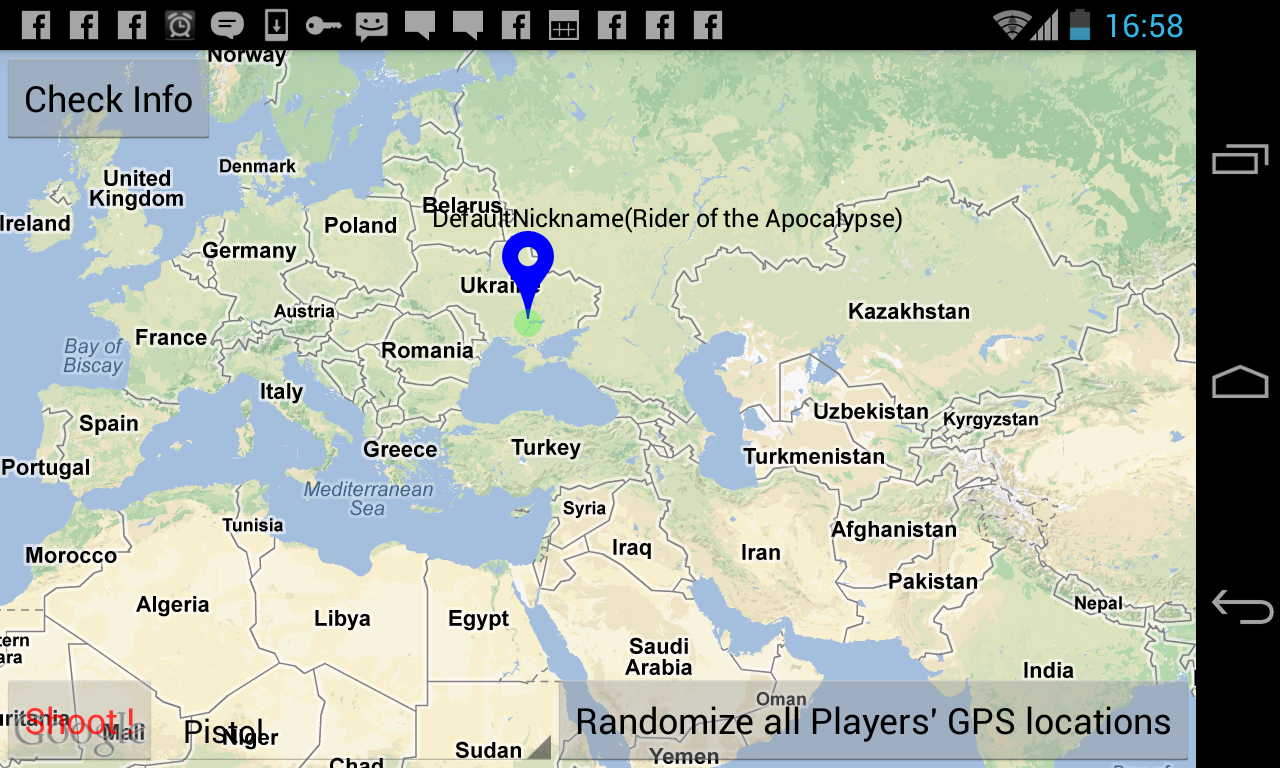
\includegraphics[height=3.5in,width=6.23in]{./images/android_screenshots/ui_prototype/UI_prototype_1.png}  
\caption{\small \sl game screen prototype \label{fig:UIPrototype1}}
\end{figure}

\begin{figure}
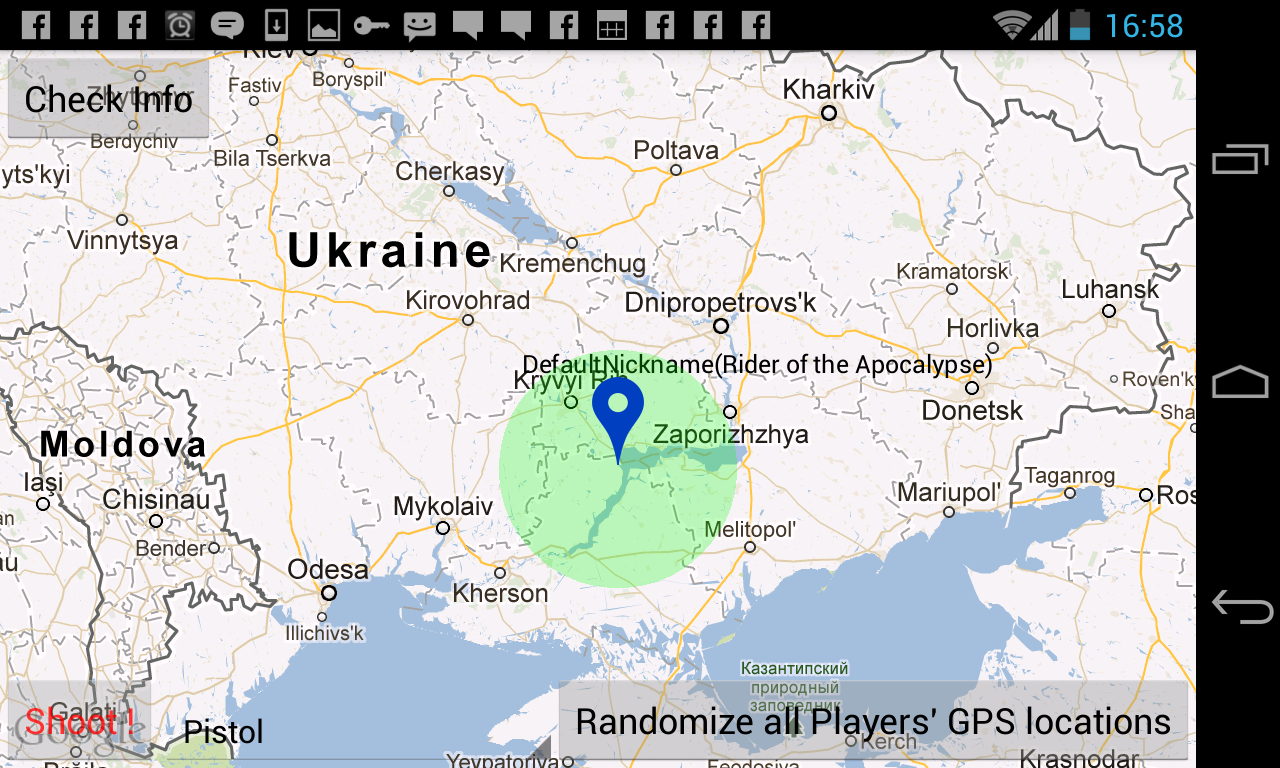
\includegraphics[height=3.5in,width=6.23in]{./images/android_screenshots/ui_prototype/UI_prototype_2.png}  
\caption{\small \sl game screen prototype \label{fig:UIPrototype2}}
\end{figure}

\begin{figure}
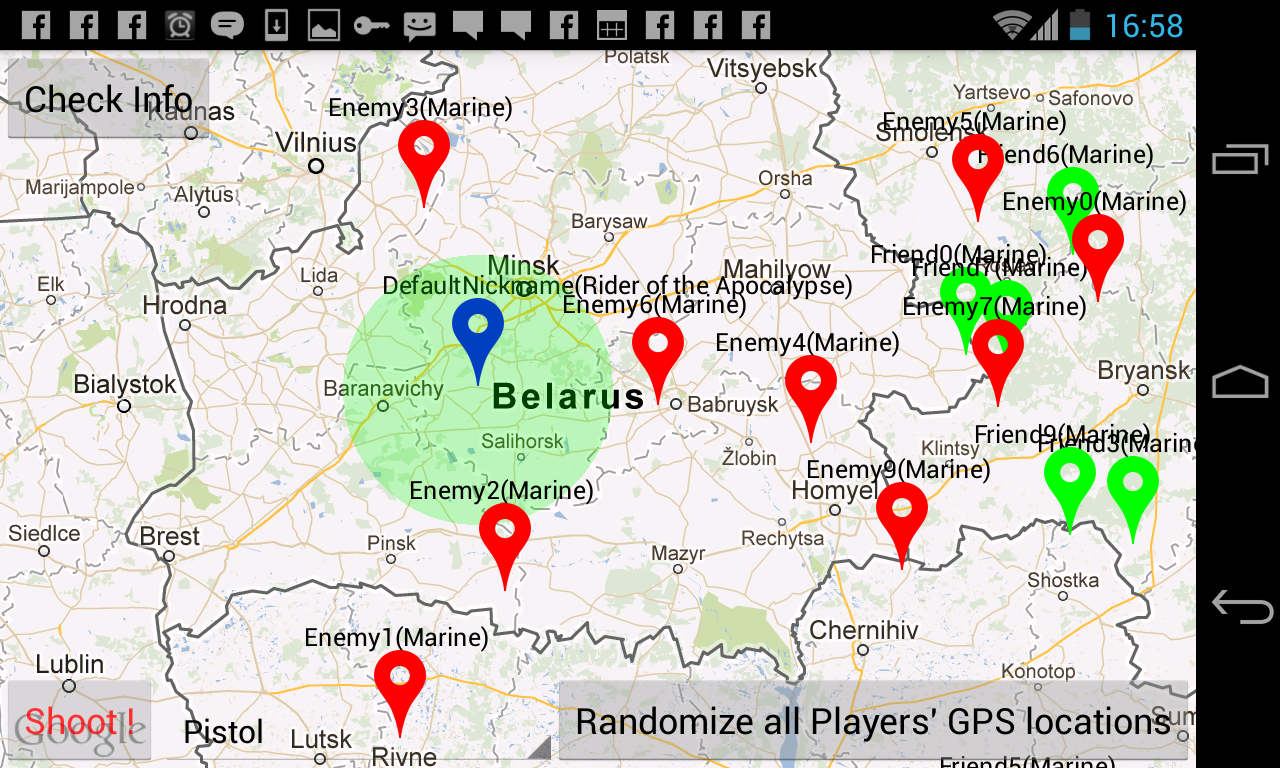
\includegraphics[height=3.5in,width=6.23in]{./images/android_screenshots/ui_prototype/UI_prototype_3.png}  
\caption{\small \sl game screen prototype \label{fig:UIPrototype3}}
\end{figure}

\begin{figure}
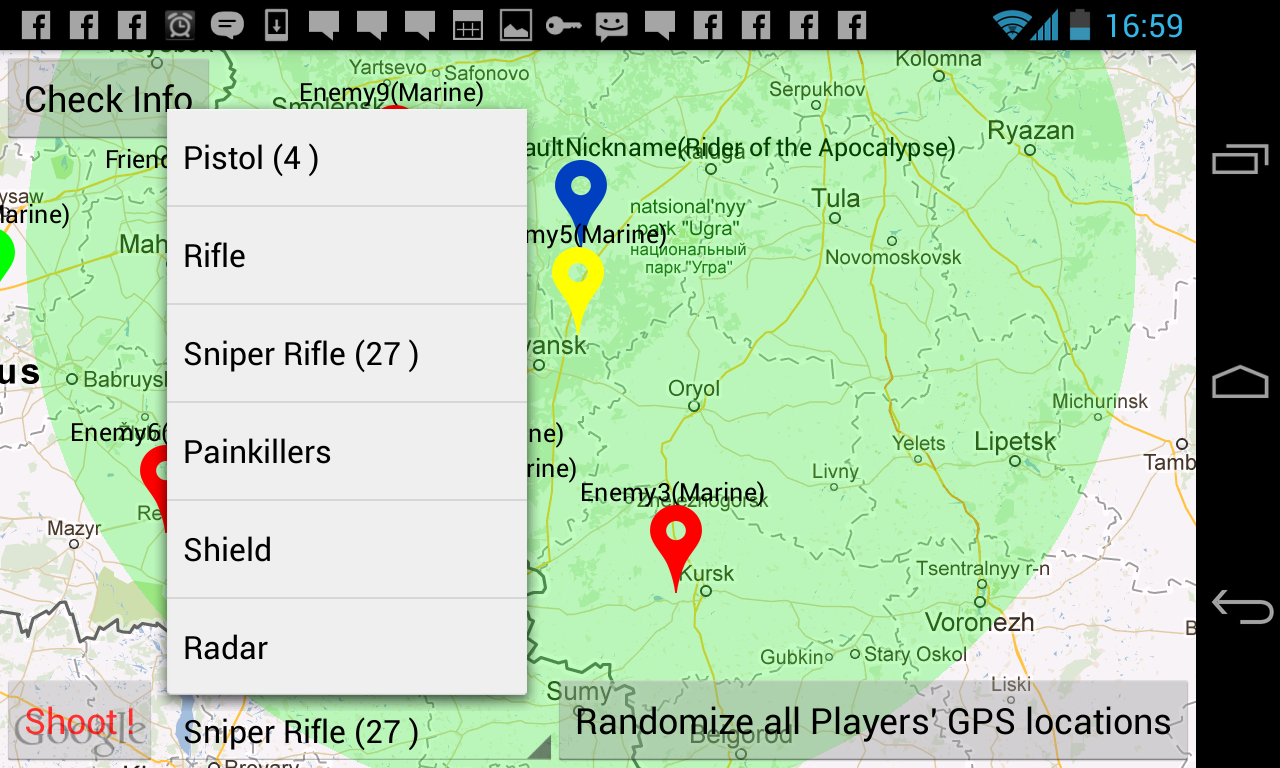
\includegraphics[height=3.5in,width=6.23in]{./images/android_screenshots/ui_prototype/UI_prototype_4.png}  
\caption{\small \sl game screen prototype \label{fig:UIPrototype4}}
\end{figure}

\begin{figure}
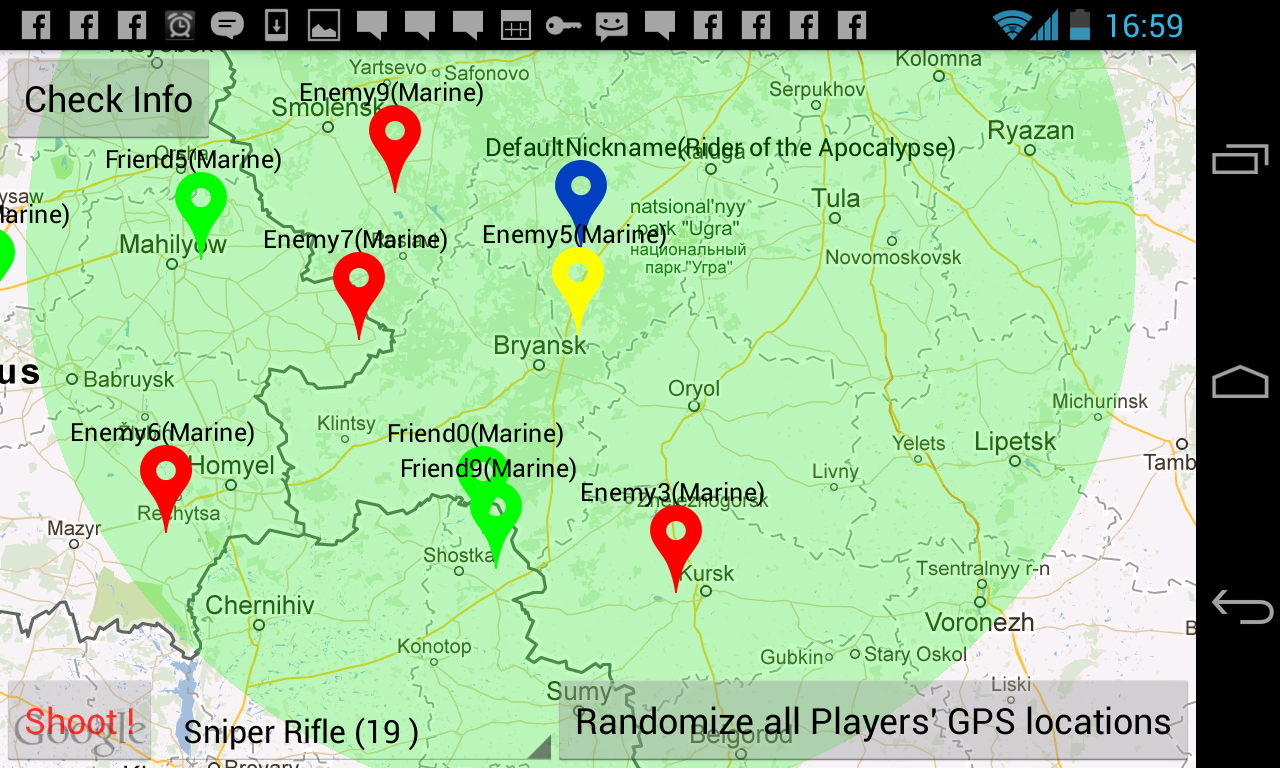
\includegraphics[height=3.5in,width=6.23in]{./images/android_screenshots/ui_prototype/UI_prototype_5.png}  
\caption{\small \sl game screen prototype \label{fig:UIPrototype5}}
\end{figure}


The creation of the game screen prototype has been followed by that of the menu
UI prototype. For starters, this one hasn't been made with easy user interaction
in mind, but rather as a set of basic functions that need to be provided
outside the game itself. Also, it has been an exercise of design. Two screens
were thought of, initially: the main menu and a lobby screen. The main menu
screen has been initially seen as only a gate to the game, an easy intro rather
than anything else. The lobby screen has been designed to functionally
accomodate what was necessary in terms of game and character preparation
- and predicted the need for another screen - that of the character settings,
marked by the presence of the button labeled 'Change my Info'. The result can be
seen in Figures \ref{fig:menuPrototype1} and \ref{fig:menuPrototype2}.

\begin{figure}
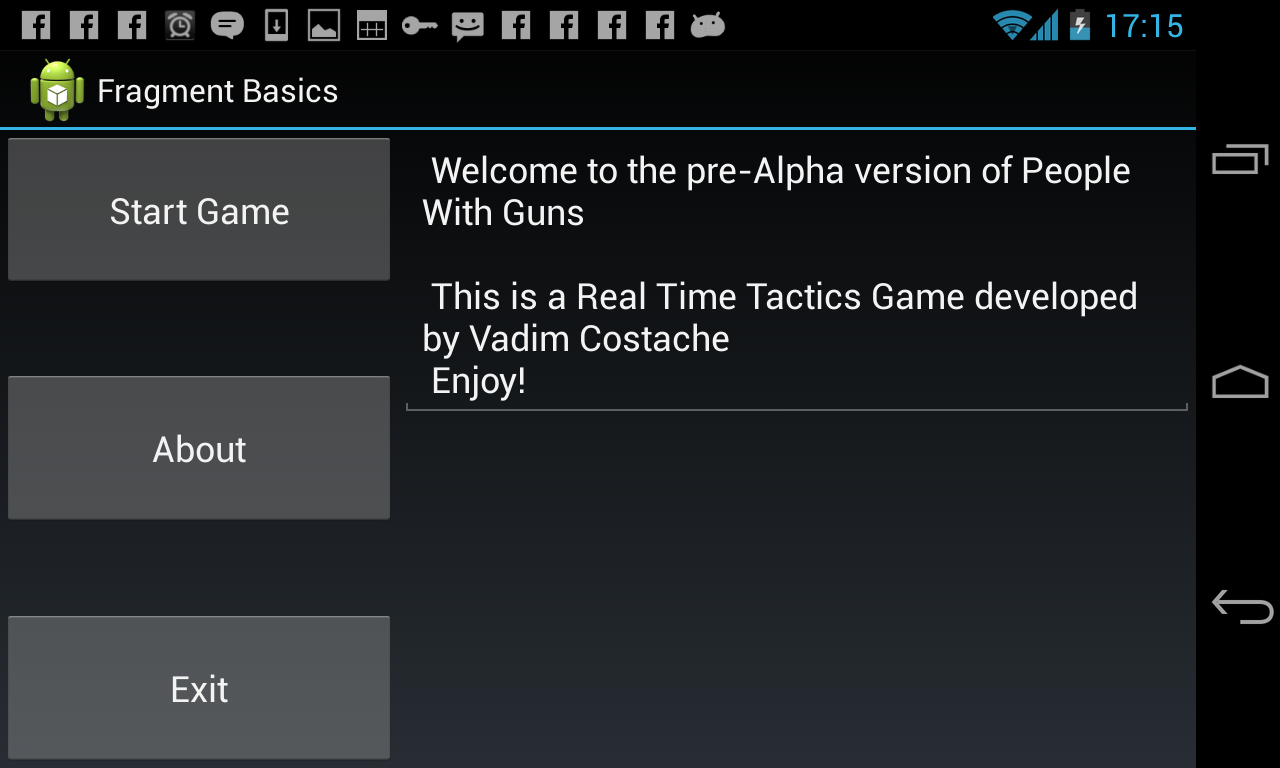
\includegraphics[height=3.5in,width=6.23in]{./images/android_screenshots/menu_prototype/MENU_prototype_1.png}  
\caption{\small \sl main menu screen prototype \label{fig:menuPrototype1}}
\end{figure}

\begin{figure}
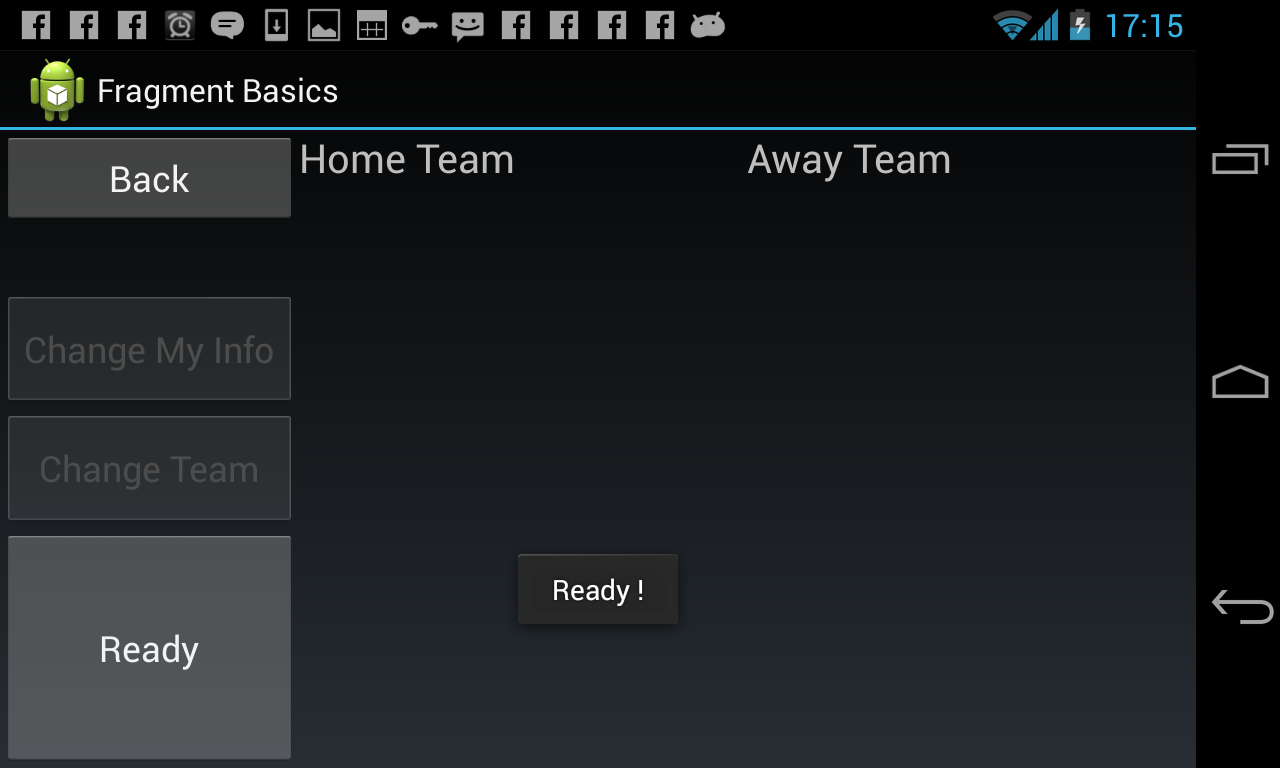
\includegraphics[height=3.5in,width=6.23in]{./images/android_screenshots/menu_prototype/MENU_prototype_2.png}  
\caption{\small \sl lobby screen prototype \label{fig:menuPrototype2}}
\end{figure}

The two prototypes have been put together in one project that has served as the
foundation of the application to come.\newline

Very soon the necessity for a settings screen right out of the main menu came up
(The server was initially run locally, on the author's laptop. The main reason
to create the settings screen was that location of the server has been changed
many times during the first stage of development - and therefore it was
necessary to re-type the IP address and port number. A button labeled 'Settings'
was added to the main menu. The settings screen came right after with just an
'OK' button and two textboxes for the IP and port inputs (as can be seen in
Figure \ref{fig:main_menu_settings}).\newline

\begin{figure}
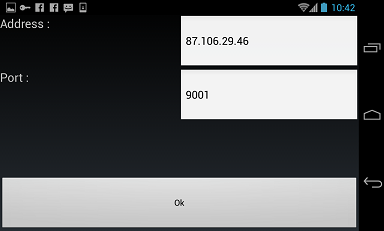
\includegraphics[height=3.5in,width=6.23in]{./images/android_screenshots/tutorial_main_settings.png}  
\caption{\small \sl The settings screen, out of the main
menu\label{fig:main_menu_settings}}
\end{figure}

At the beginning of the development, as functionality to connect to the server
has just been implemented, there was no loading screen. Instead, the application
UI would just freeze for a few thousand milliseconds. That has been considered
unacceptable from a usability perspective. The first idea was to add a loading
widget on top the main menu screen - but the separate loading screen has proven
itself a more versatile concept that can be used for functionality to come. The
loading screen had to mark the transition to entering the game. A loading screen
was added, with a simple loading widget looping infinitely and a 'Loading' text
at the bottom of the screen(Figure \ref{fig:loading}). This screen has remained
visually untouched until the last version of the application.\newline

\begin{figure}
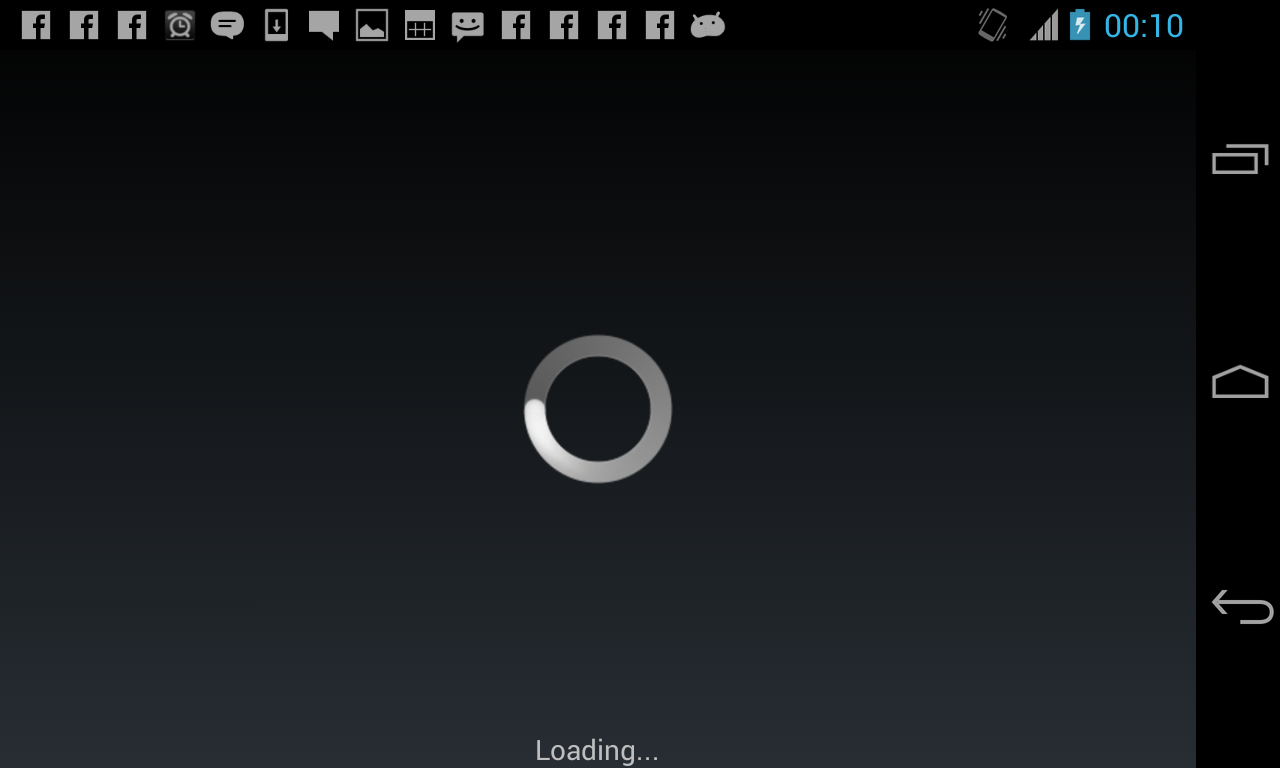
\includegraphics[height=3.5in,width=6.23in]{./images/android_screenshots/tutorial_loading.png}
\caption{\small \sl The loading screen\label{fig:loading}}
\end{figure}

Once the game client became capable of successfully connecting to the server and
setting up everything for the lobby screen, the need for the lobby settings
screen came up - and therefore the lobby settings fragment has been created -
with a spinner for choosing between characters, a textbox for the nickname, a
multiline textbox for loading the description of each character or 'profession'
and an 'OK' button. This screen has also remained largely unchanged until the
current point of development and can be observed in Figures
\ref{fig:lobby_settings_1} and \ref{fig:lobby_settings_2}.

\begin{figure}
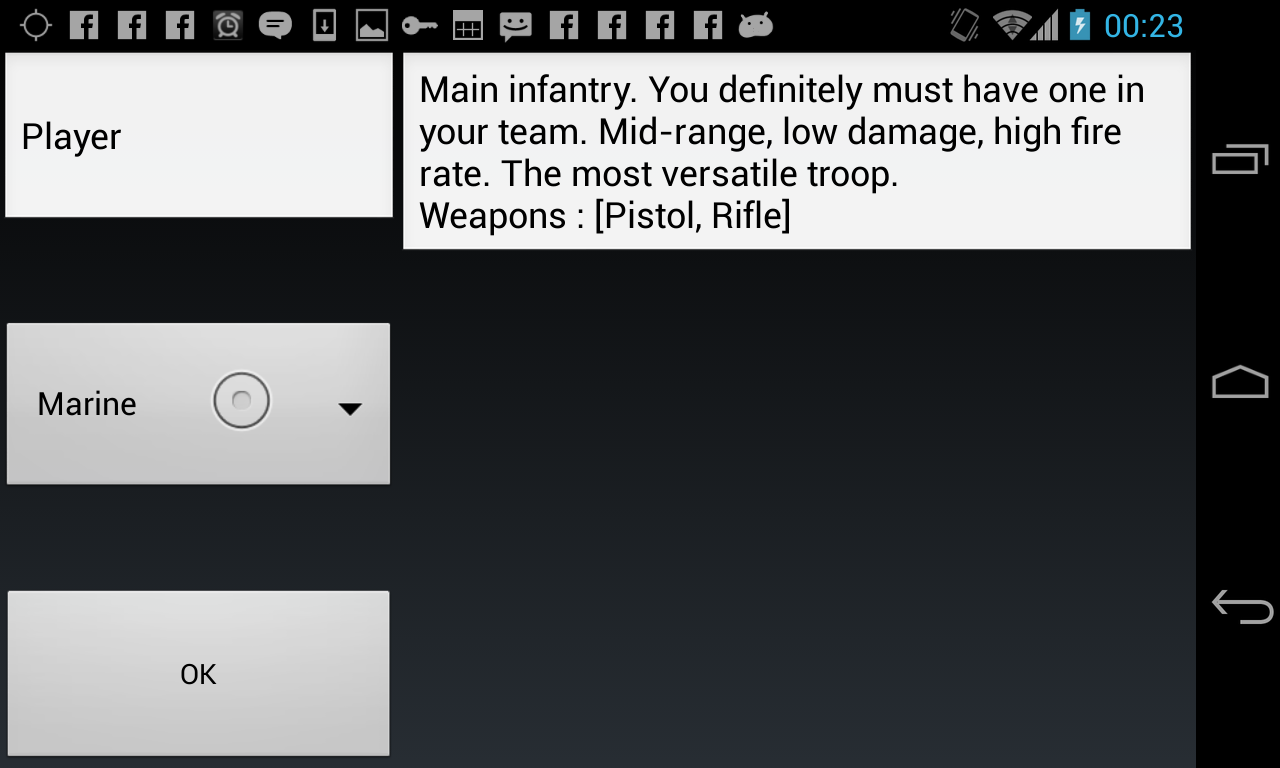
\includegraphics[height=3.5in,width=6.23in]{./images/android_screenshots/first_development/game_first_development_9.png}
\caption{\small \sl The character editing screen (a.k.a. the lobby settings
screen) menu\label{fig:lobby_settings_1}}
\end{figure}

\begin{figure}
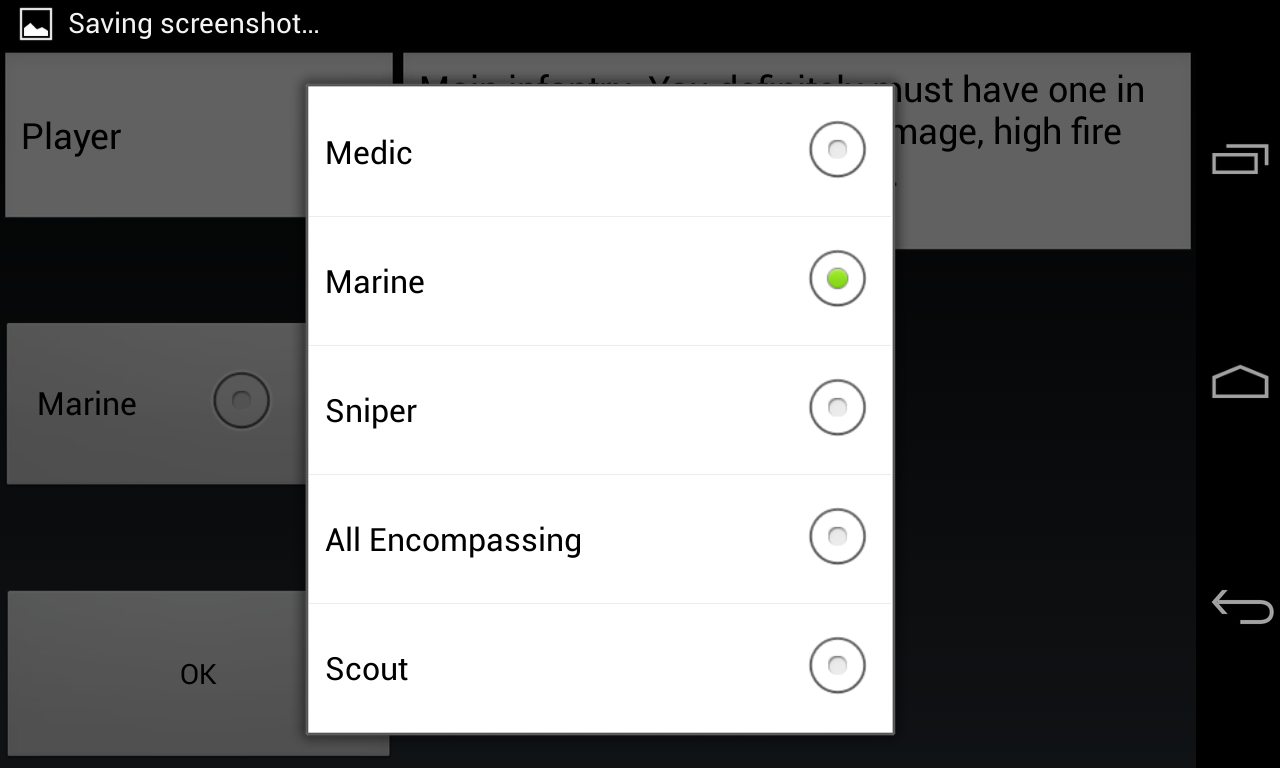
\includegraphics[height=3.5in,width=6.23in]{./images/android_screenshots/first_development/game_first_development_10.png}
\caption{\small \sl The character editing screen (a.k.a. the lobby settings
screen) with the character selection dialog opened
menu\label{fig:lobby_settings_2}}
\end{figure}


\subsection{The first testing phase}

Contrary to the original plans, the first testing phase took only half a day
with another half day of preparations. Prior live tests have been done by the
author alone, with two phones.\newline

Five people (three male and two female) were invited to play the game. Three of
them had Android phones. The other two have used the two phones that the author
had in posession at the time. Unfortunately, most of them had Android 2.2 and
2.3 installed. The preparations meant convincing them to volunteer their phones
for an OS upgrade. Android 4.0 was installed.\newline

The tests have been done mostly indoors, as they revealed various bugs in the
server and client code that were not detected when testing discrete features.
Because six people had five phones, two of them have played
alternatively.\newline

Because not all players had 3G connections available, the game has been played
by connecting to a WiFi router. The first bug we noticed was that occasionally
the game would disconnect for no apparent reason. Others have been related to
GPS devices in one of the phones not retrieving the position and crashing the
application or concurrency issues improperly treated.\newline

A few temporary quick fixes got the game working and the testers managed to play
the game, firstly indoors for a few times and then outside, while still
connected to the WiFi router. This has inadvertently been a test of the WiFi
coverage of an average old 802.11 b/g router - around 50 - 70 meters radius in
an open space describing a half-circle around the router. The author was the
first to accidentally run outside the WiFi coverage and get disconneted.\newline

After the playing was finished, the testers and the author sat down for a
focus group discussion, during which criticism of the gameplay, UI and game
satisfaction were expressed. Although the concept itself has been positively
appreciated, the game UI has received a lot of criticism. Also the random
disconnection of the game from the server has caused a lot of frustration among
the test players. A proposal has been made to allow saving the last player
status and position on the server and allow a timeout until the player would not
be allowed to reconnect. A debate led to the conclusion that enabling such a
feature could allow cheating: A player would disconnect from the game, get close
to other players, reconnect, shoot and repeat the sequence - thus avoiding
damage and causing frustration to others. \newline

Until the end of the first testing session done with a group of people, the UI
has remained largely untouched. The two unused buttons on the game screen have
been kept for tester feedback on how pleasant the position of those buttons is
for the reach of their fingers. The goal for the game UI has been to become
similar to a game controller, while having the game screen in the middle. And
the screen had to be layed out in a way in which the user would not feel cramped
when playing the game. The only addition to the UI has been the 'Settings'
button in the main menu, together with the settings screen.\newline

The first people to test the game have criticized the following aspects:
\begin{enumerate}
  \item \textbf {The game UI}: The need to reselect the target every time the
  weapon is switched has proven frustrating. The entire process of selecting
  a weapon before firing it has been regarded as too slow: the players wanted to
  be able to shoot the entire arsenal immediately, if possible.\newline
     
  The lack of control over what is happening has been criticized: The player
  health was only displayed above the head of the player, along with the name
  and 'profession'. It made it hard for players to notice changes. Notifications
  on who 'shot' who were not yet implemented. The player's health was not
  displayed anywhere. Messages could not be sent to the team. The first proposal
  has been to enable writing and sending messages, messenger style. After some
  discussions, the conclusion came that predefined messages are much more
  useful(like the ones used in the video game ''CounterStrike''), while more
  complex messages can be communicated verbally, keeping the players more
  focused on the dynamics, rather than on the technicalities of the game.
  
  \item \textbf{The menu UI}: The lobby UI has been criticized - but not for
  it's layout, but for the comprehensibility - there was no mark for the
  player's 'Ready' status, the 'Change my Info' label wasn't comprehensible. The
  nickname and 'profession' were not remembered from one game session to the
  other or from one app launch to the other. This frustrated the users - and
  they simply refused entering their nicknames after a few games. The game ended
  up with no one knowing who's who, because they had the same nickname - the
  default 'Player'. One tester complained that he wanted to click his own name
  in the team lists and get to the settings screen - but functionality
  to do that was not implemented.\newline
  
  A general complaint has been expressed towards the fact that there are no
  tutorials on how to play the game.
\end{enumerate}

The first testing phase, though short, has left a lot of guidelines on what to
do from that point on.\newline

\subsection{The second develpment phase}

The first testing phase has left a lot of 'todos', notes and guidelines for
better adapting the UI and game mechanics to the player's needs. The second
development phase has addressed these needs with a personal touch from the
author and an influence of the switch to a newer version of Maps API (V2). The
newer version of Maps API also came with the requirement that Google Play
Services be installed on each device that runs the game.

\subsubsection{The Server}

The only change done on the server in the second development phase, beyond bug
solving, has been the switch from InetAddress to InetSocketAddress as key in the
server's management HashMaps. That's because multiple connections from behind a
router with NAT were not possible. InetAddress only holds the remote IP of the
connection. The InetSocketAddress now holds both the IP address and port number
of the connection.

\subsubsection{The Client}

We will describe the changes made to the client, after the first testing phase.
The most important set of changes has occured on the UI: The Google Maps V1 API
has been discarded in favor of the V2 API, the appearance of the UI has been
radically changed and most of the back end functionality that served the game
screen has been discarded and rewritten.

The client now uses seven fragments for the UI: 'Main Menu', 'Info and
Tutorials', 'Settings', 'Lobby','Lobby Settings', 'Loading' and 'Game':

\begin{enumerate}
  \item 'Main Menu' : It has been slightly modified: The 'Start Gane' text has
  been changed into 'Connect to Server' - making its functionality more
  obvious. The logo presented in Figure \ref{fig:game_logo} has been added for
  user feedback. The 'Info and Tutorials' button has been added - it leads to
  a new Fragment that presents the idea and functionality of the game.
  
  \item 'Info and Tutorials' is a screen with a number of buttons and a
  scrollable view for displaying text and images. Here, the user will find
  instructions for the purpose how use of the app and detailed descriptions of
  the functionality of the 'Lobby' and 'Game' UIs.
  
  \item 'Settings' has not been modified.
  
  \item 'Loading' has not been modified.
  
  \item 'Lobby' : it has been slightly modified to remember the last used
  nickname and 'profession'. Each player in the team lists now shows the ready
  status of that player and a '\[ME\]' indicator has been added to the current
  player so that he can identify himself in the list. Clicking on one's own
  nickname in the list now navigates to the 'Lobby Settings' screen for
  nickname and 'profession' change. Two background images have been tried out on
  this fragment, for user feedback. They are shown in Figure
  \ref{fig:game_background_black} and Figure \ref{fig:game_background_white} 
  
  \item 'Lobby Settings' has not been modified. A background image has been
  tried out as background, for user feedback. See Figure
  \ref{fig:game_background_lobby_settings}
  
  \item 'Game' has been completely modified. Due to tester feedback and
  the change of the Maps API, it has gone through radical changes. At this
  point, the game screen looks as follows: for all the 'weapons' and 'powerups',
  buttons are aligned starting from the bottom left corner of the screen until
  close to the bottom right corner. From the bottom right corner upwards, on
  the vertical axis, three buttons and a TextView have been placed: the
  'Previous Target', friend/foe toggle, 'Next Target' buttons and a TextView
  that shows the distance from the current player to the selected friend or
  foe. If no player is selected, the presented text will be '0(Self)'.
  Otherwise, just the distance measurement is shown, with no text. In the top
  right corner, the default 'My Position' button is shown - with its specific
  icon. In the top left corner of the screen, a TextView with large text
  indicates the 'health points' of the player. Underneath the health indicator
  lays a Spinner for sending predefined messages to the team. The full
  functionality of the UI will be presented below.
  
\end{enumerate}

The typical app use scenario goes as follows: The player enters the game and
sees the 'Main Menu'. The application checks if Google Play Services are
installed and if the GPS is turned on. If either of these conditions is not met,
a dialog is presented: the player must choose to install Google Play Services and/or turn on
the GPS or exit the game. Each dialog directs the user to the appropriate Google
Play or Settings page - where the player only has to either click 'Install' or
switch the 'Enable GPS' toggle to 'ON'.\newline

Once there are no more requirements to be met in order to play the game, the
player can click on 'Connect to Server', be briefly presented with the 'Loading'
fragment and then enters the 'Lobby'. There, if the app was started for the
first time, he can see the default nickname 'Player' and the default
'profession' - Marine. If the app was previously used, the player will see the
last nickname and 'profession' used in previous runs. The server distributes the
players according to team sizes, so the player has an equal chance to see
oneself in either the 'Home' or 'Away' team. Then, the player can opt to change
the team by using the 'Change Team' button. Also, the nickname and 'profession'
can be changed by navigating to the 'Lobby Settings' screen. Once the 'Ok'
button is pressed in the 'Lobby Settings' screen, the changes are saved by the
application and sent to the server for broadcasting, and the player is returned
to the 'Lobby' screen.\newline

At the point where all the players have done setting up, they can send the
'Ready' signal. When all the players are ready (for testing purposes, one
player present on the server is enough to start a game), the five second
countdown is received from the server and the player is now facing the 'Game'
screen.\newline

In order to understand what can be done at this point, a detailed description of
the 'Game' UI is necessary: \newline

We can visualize the UI based on the screenshots presented in Figure
\ref{fig:game_ui} and Figure\ref{fig:game_ui2}. It presents the groups of UI
elements on the screen.
We shall now present all of them, separated into groups, by position
(positioning also separates functionality groups, therefore we can also state
that they are presented by related functionality). All the UI elements on the
'Game' UI are programmatically generated - and not from an XML file  :
\begin{enumerate}
  \item\textbf{The bottom of the screen, starting from the bottom-left corner}:
  The 'weapon'/'powerup' buttons are generated once the 'Game' fragment is loaded,
  based on the list of weapons specific to the player's 'profession'. They
  appear from left to right. If less or equal to three weapons are given, the
  buttons will be made slightly larger than otherwise - up to a maximum of six
  (the number of weapons featured in the test 'profession', 'All Encompassing').
  Each button press shoots the 'weapon' or 'powerup', according to a so-called
  'policy' provided in the Weapon object. The policies are as follows: 'self',
  'friends', 'friends and self', 'enemies', 'friends and enemies', 'friends and
  enemies and self'- stating on which kinds of players one given 'weapon' or
  'powerup' can be used. A button long press will draw the range of the
  'weapon'/'powerup' on the map, with the player's position in the center.
  
  \item\textbf{The bottom-right corner of the screen}: The player selection
  buttons and the distance indicator are generated on the vertical axis, starting from the
  bottom-right corner of the screen - in order, the 'previous target',
  friends/enemies toggle, 'next target' buttons, and on top a TextView showing
  the distance to the selected player or '0(Self)' if no player is selected(in
  translation, the 'self' or 'current player' is selected). The friends/enemies
  toggle is used for switching choosing between the two groups of players:
  friends or enemies. On each press on the 'next target' button,
  the next closest player from the chosen category is selected. The reverse
  applies to the 'previous target' button - which selects the previous farthest
  player if a player is selected and the closest one otherwise. The distance
  indicator serves for the use of an experienced player who knows the weapon's
  distances by heart and does not need to draw the weapon range circle on the
  map. The players may also be selected by simply tapping their respective
  markers on the map - but through testing it has been determined that in a more
  intense and dynamic situation, selection by clicking on the marker can become
  difficult and inaccurate. Both modes are supported now. At this stage of
  development, deselection of players (and implicit selection of the current
  player) is done by touching a random unoccupied area on the map.
  
  \item\textbf{The top-right corner of the screen}: The 'my position' button - 
  Clicking it will cause the map to be automatically scrolled until the position
  of the current player is centered.
  
  \item\textbf{The top-left corner of the screen}: The health indicator is a
  TextView that presents in large text the available health points of the
  current player. Underneath it lies a spinner that provides a list of messages
  that the player can send to his/her team. One can do so by clicking on the UI
  element representing the spinner, beneath the health indicator. After the
  first click, the spinner dialog appears and shows the list of messages. The
  player can send one of the messages in the list by clicking it. The dialog is
  canceled by selecting a message or clicking outside it.
  
  \item\textbf{The area in between the two top corners of the screen}: This is
  the area where the powerup duration is dynamically shown during its effect.
  This can be seen when the player casts 'invisibility' or 'shield' on oneself
  or when a friend casts 'shield' on the player.
  
  \item\textbf{The area above the weapon buttons}: This is where the
  notifications appear, in the form of Toasts. By default, a toast has a given
  lifespan - but each time a new toast needs to be displayed, it first closes
  the toast currently on display, if it is the case.  
\end{enumerate}

Although they are not yet discretized, thus far we can distinguish three types
of game that can be played with the current setup: the \textbf{Default
game}(which requires multiple players, but excludes the 'All Encompassing' game
type); \textbf{Duel}(two players choose the 'All Encompassing' profession -
receiving the entire arsenal provided by the game - and try to eliminate
each other from the game by using various strategies of combining 'weapons' and
'powerups'); \textbf{David vs. Goliath}(a small number of players choose the
'All Encompassing' profession and play against a significantly larger number of
players that use all the professions except 'All Encompassing').\newline

Until now, the default game and the duel have been tried out - and they are
fit for different situations: The default game can take up to 20 minutes and is
played on a large area (there is no limit for now), depending on the mood and
disposition for running of the players. The duel is performed usually by two
players sitting next to each other and takes two-three minutes.\newline

Thus far, no game end condition has been introduced - players who lose all
health points are notified that the game is over for them through a dialog that
gives them two options: quit the game or spectate. The second option implies
that they are marked as 'dead' on the map, cannot be selected and their weapon
buttons are removed from the screen. Still, they can watch the evolution of the
game on their mobile devices. When all players of one team are marked as 'dead'
(they have lost all their 'health points') and at least one member of the
opposing team still has more than zero health points, it can be considered a win
for the opposing team. The ending condition has not been implemented, because
for this stage of development of the application there is no reward system
implemented. \newline

The main functional differences from the first development of the game are:

\begin{enumerate}
  \item A switch from Google Maps API V1 to V2 has been done. This implied
  rewriting the whole UI and several methods in the helper libraries.
  
  \item Because of the switch mentioned above, the custom Overlay object (along
  with the custom tap and marker drawing functionalities) and the object
  responsible with position retrieval have been discarded. Position retrieval is
  done through an option provided by the GoogleMap object provided by the Google
  Maps V2 API. The whole marker and weapon range drawing are also done through
  the GoogleMap object - OverlayItem objects have been replaced by Marker
  objects and GeoPoints have been replaced by LatLng instances.
  
  \item The whole UI has been rewritten, having as a result what was described
  above.  
  
\end{enumerate}

Passive disconnection detection functionality has been added in the loop that
waits for incoming messages. The functionality of some weapons and powerups has
been modified. A powerup called `Radar` that was present in the first
development iteration, but did nothing has been removed. The 'Invisibility
cloak' and 'Knife' have been added. Powerup duration indicators have been
added.\newline

The final message structure in between the server and the client will be
presented in one of the Annexes.\newline

During the second development phase, a lot of decentralization and
modularization of functionality has been done. Some classes that only served the
Game UI relying on Maps API V1 have been removed. Others, serving the Maps API
V2 have been added. Various bugs that caused crashes have been corrected. The
starting condition has been reintegrated in the game - the weapon buttons
are disabled until a 'Start Game' signal is received from the server.\newline

\subsubsection{Logging, Testing and Data Usage}
After the first testing phase, a the need of a logging system was felt. A
logging system based on Logcat capture has been added. Uncaught exceptions are
now caught and logged before the app closes. \newline

A lot of testing has been done with the 'UI/Application Exerciser Monkey' to
show up potential bugs and crashes. Some bugs have been found and patched - but
one has persisted: Apparently, there are some humanly-impossible combinations of
keyboard and touch inputs that lead to a Spinner dialog crashing the
application. This is an Android-related issue and cannot be solved by
the author.\newline

Another bug that has persisted is that of the WiFi disconnection(3G connections
stay alive). Apparently, this is an Android bug.\newline

As for logging, a Logger class has been created, its functionality has been
extended to retrieve the data usage of the app. Because of various compatibility
reasons, the data usage of the entire device during the usage of the app is
retrieved, instead of the usage of the application itself. This means that the
data usage of, say, social network or mail applications adds to the count - but as a
general idea (and not very precise numbers) is needed, it has been considered a
decent solution.

\subsubsection{The UI}

The second development session has come with the mindset to completely change
the UI. And not only that was done: the whole underlying framework has been
changed. A switch to the Google Maps V2 API was made. A lot of functionality has
been thrown away - such as the Overlay that served for drawing the players and
for laying out the controls. A lot of new controls had to be added. A lot of
underlying technicalities have been changed(such as the custom screen tap
functionality and data objects used for positioning).\newline

Because of the switch to the new Maps API, the MapView object which served as
the container for all controls has disappeared. It has been replaced by a
GoogleMap object which is not intrinsically a View and cannot be treated thusly.
Some improvisation was required to artificially create a container for the map.
This has been done by programmatically creating a RelativeLayout and adding the
View that contained the map as a child. Then, the apparent choices have been to
either add all the controls programmatically - which is very tedious - or embed
a Fragment within another Fragment - which is bad for performance. All the
controls have been generated and added programmatically. And the result has been
previously described in the paper - having as a result the UI presented in
Figure \ref{fig:game_ui2}: The UI has been properly partitioned in four
functional areas that, although they provide much more control and
functionality, they don't cloister the map. The health of the current player is
visible, a button has been added to center the image on the current position of
the player, individual buttons are generated for the list of weapons provided
for a 'profession', a group of buttons is added for help in target selection.
Target selection by tapping on the screen has been preserved as an alternative
to the selection buttons. The latest addition - the Spinner serving message
sending was taking up too much space and hindered the view of the map. A good
solution has been to make it semi-transparent - thus, making it non-intrusive,
yet present. The ranges of the weapons are now drawn in green on demand, by long
pressing the weapon buttons. The blue circle around the player's position is the
default indication of the GPS accuracy. Thus far, it has not been removed - as
it can be useful in various gameplay situations.\newline

\begin{figure}
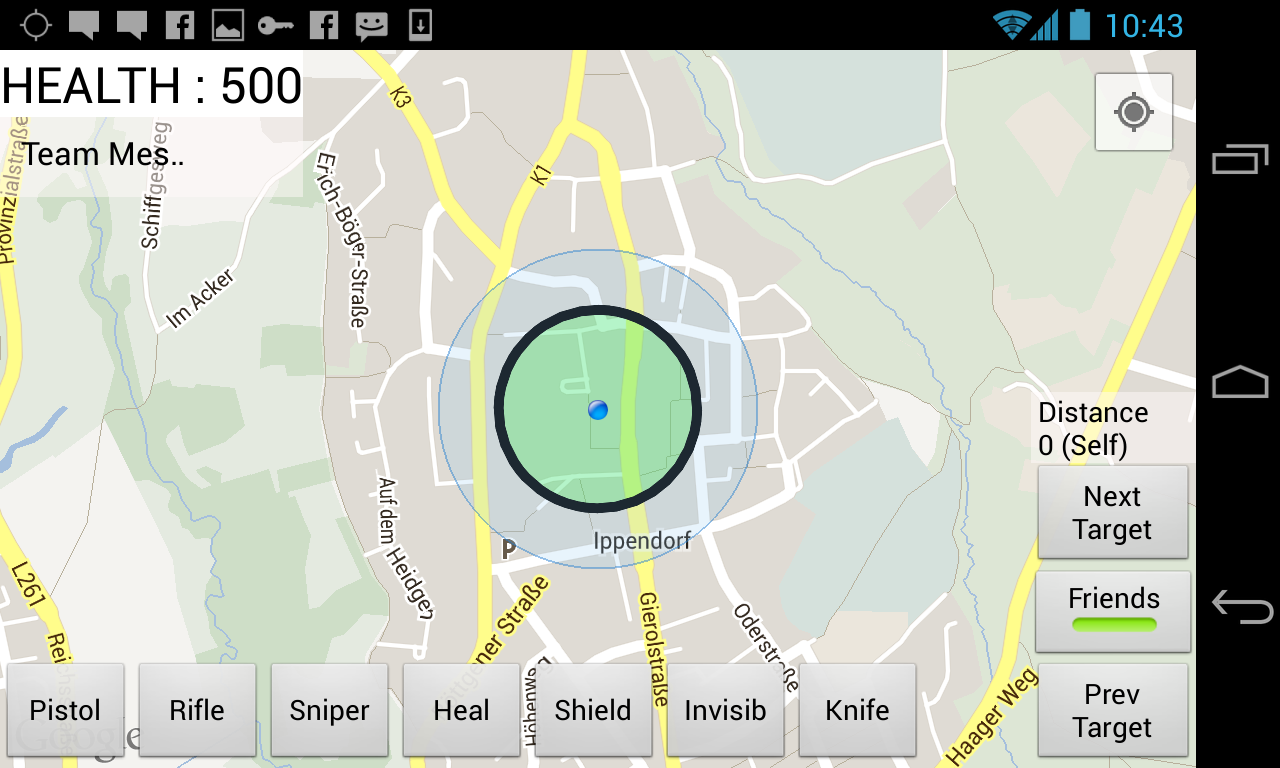
\includegraphics[height=3.5in,width=6.23in]{./images/android_screenshots/second_development/game_second_development_5.png}
\caption{\small \sl The game UI \label{fig:game_ui2}}
\end{figure}

The menu UI has also been modified:
\begin{enumerate}
  \item \textbf{The main menu screen}: The welcome message has been removed and
  place has been left for a potential logo. The addition of a logo has been
  attempted, as seen in Figure\ref{fig:logo_white}. Also, a button to navigate
  to the newly added info and tutorials screen has been added.
  
  \begin{figure}
  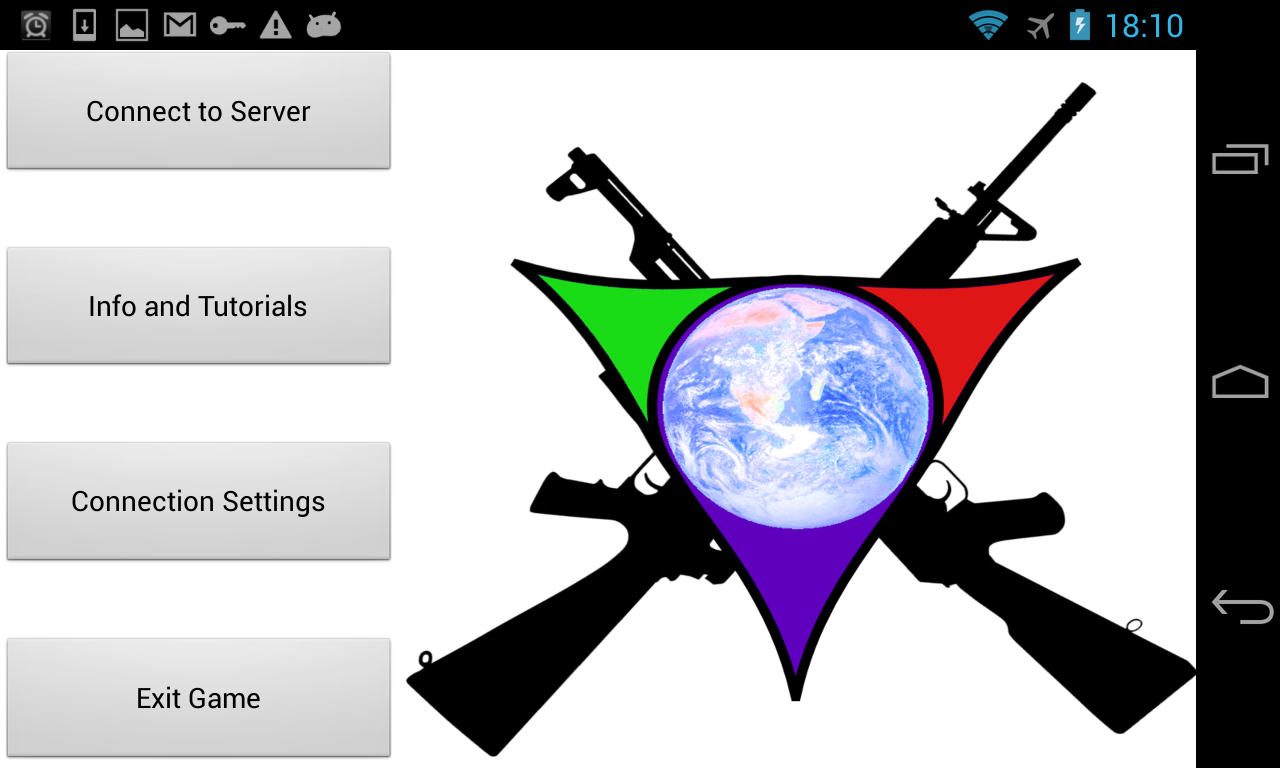
\includegraphics[height=3.5in,width=6.23in]{./images/android_screenshots/logo_white.png}
  \caption{\small \sl A white game logo \label{fig:logo_white}}
  \end{figure}
  
  \item \textbf{The info and tutorials screen}: A new screen has been added.
  It contains four buttons that lead to information and tutorials on what the
  game is and how to play it. The initial plan was to have a WebView as
  container and load the tutorial articles in HTML format. Then a simpler
  solution was devised and instead of the WebView, a ScrollView was added as
  container and a LayoutInflater object is now used to generate the
  tutoarial articles from XML files. The results can be seen in Figures
  \ref{fig:tutorial_fragment1} and \ref{fig:tutorial_fragment2}.
  
  \begin{figure}
  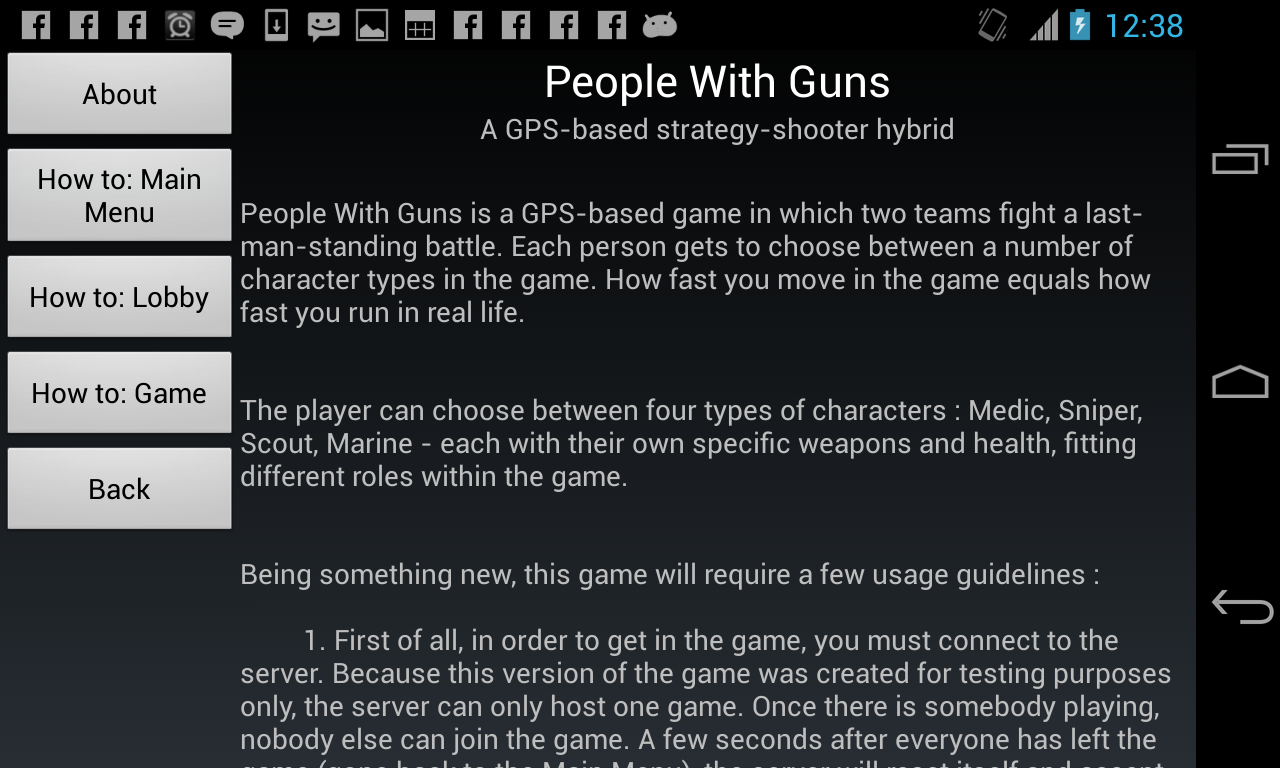
\includegraphics[height=3.5in,width=6.23in]{./images/android_screenshots/tutorial_fragment_1.png}
  \caption{\small \sl Tutorials screen: the About
  page\label{fig:tutorial_fragment1}}
  \end{figure}

  \begin{figure}
  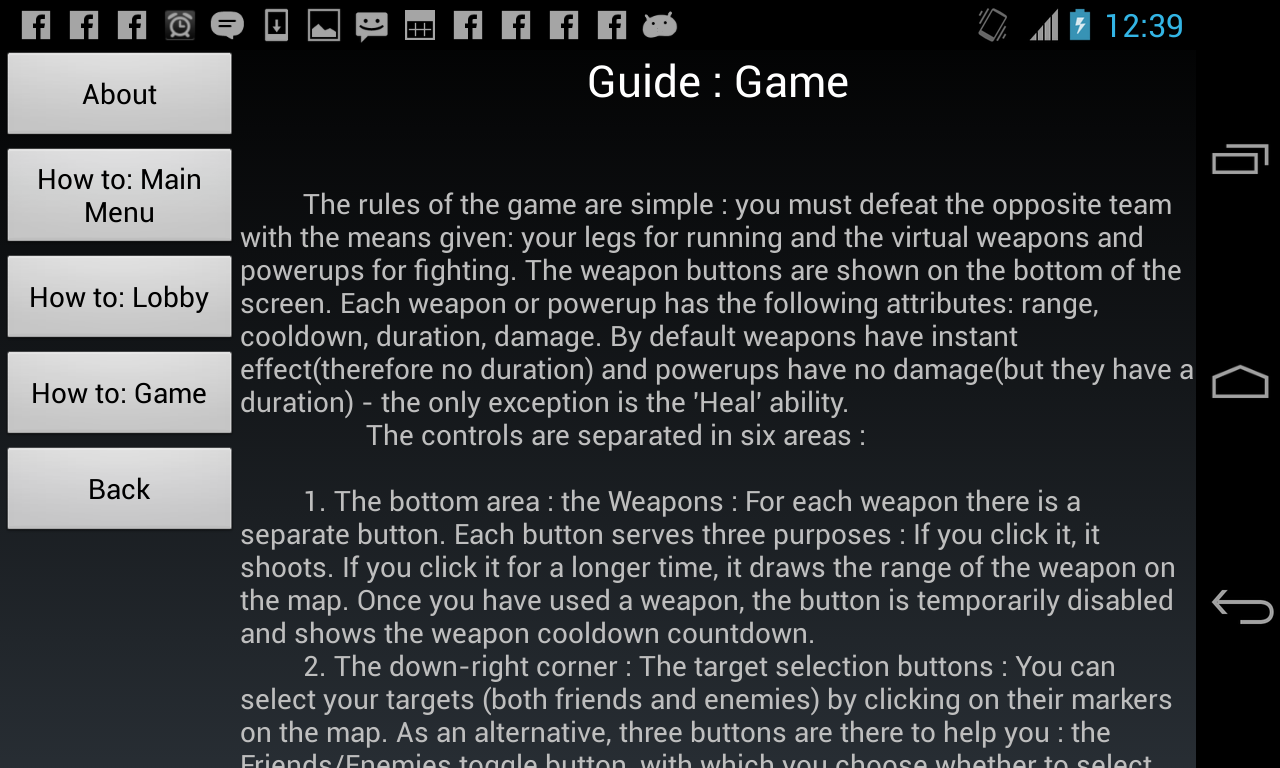
\includegraphics[height=3.5in,width=6.23in]{./images/android_screenshots/tutorial_fragment_2.png}
  \caption{\small \sl Tutorials screen: the Game Guide page
  \label{fig:tutorial_fragment2}}
  \end{figure}
  
  
  \item \textbf{The lobby screen}: The lobby screen was also modified: The
  requested feature to map the click on one's name to the character settings
  screen was implemented. Also, the ''ME'' marker has been added to distinguish
  the current player from the rest and the ''READY'' marker of one's 'Ready'
  status. Two backgrounds have been tried on this screen, as seen in Figures
  \ref{fig:lobby_background_black} and \ref{fig:lobby_background_white}.
  
  \begin{figure}
  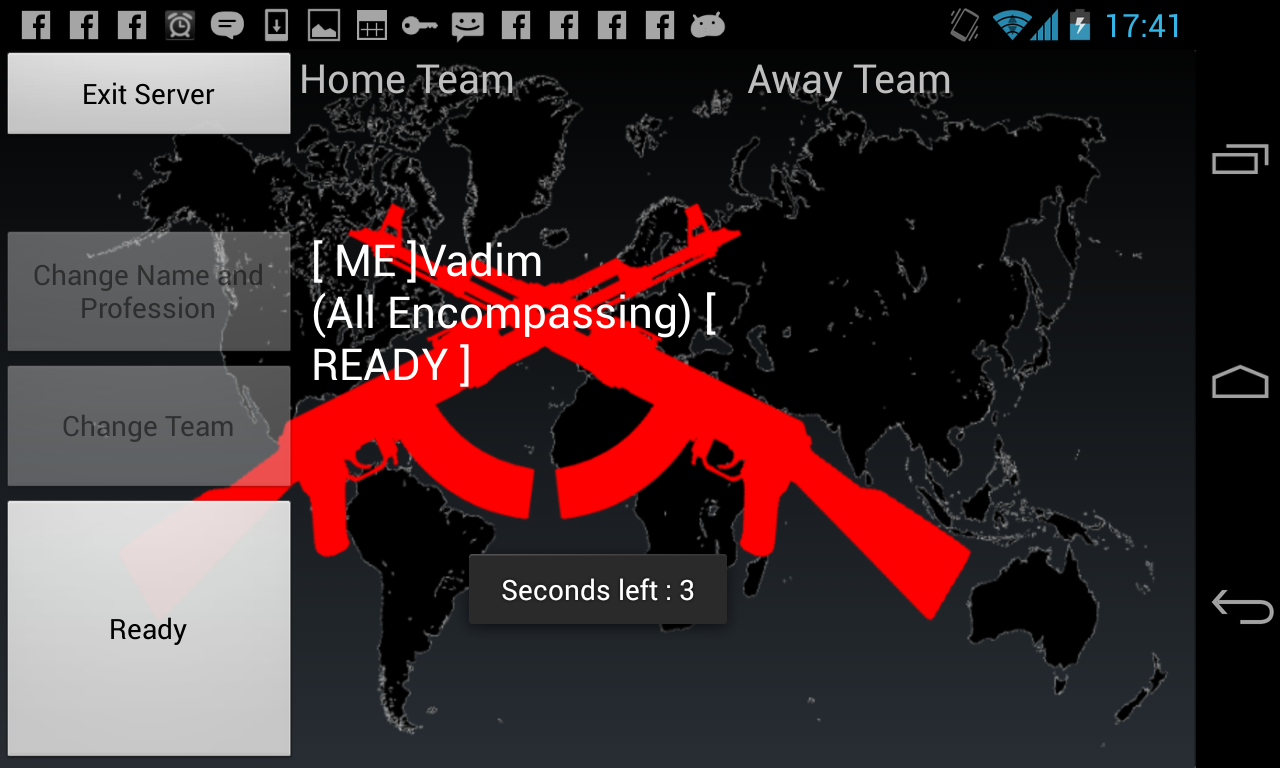
\includegraphics[height=3.5in,width=6.23in]{./images/android_screenshots/second_development/game_second_development_3.png}
  \caption{\small \sl Lobby screen with black background
  \label{fig:lobby_background_black}}
  \end{figure}

  \begin{figure}
  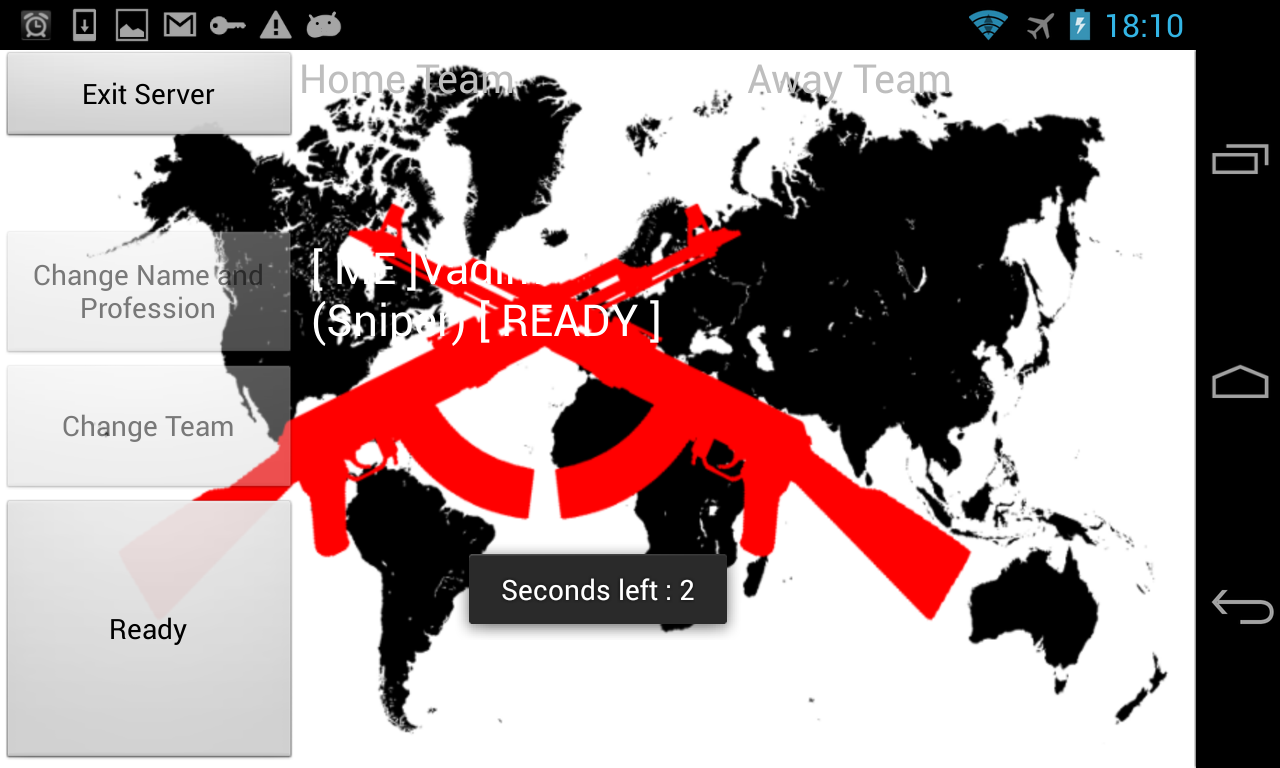
\includegraphics[height=3.5in,width=6.23in]{./images/android_screenshots/lobby_background_white.png}
  \caption{\small \sl Lobby screen with white background
  \label{fig:lobby_background_white}}
  \end{figure}  
  
  \item \textbf{The lobby settings screen}: The lobby settings screen has been
  kept almost intact since its creation. The functionality to remember the last
  used player's nickname and 'profession' was added. Also, two backgrounds in
  black and white have been tried out. They can be seen in Figures
  \ref{fig:lobby_settings_background_black} and \ref{fig:lobby_settings_background_white}.
  
  \begin{figure}
  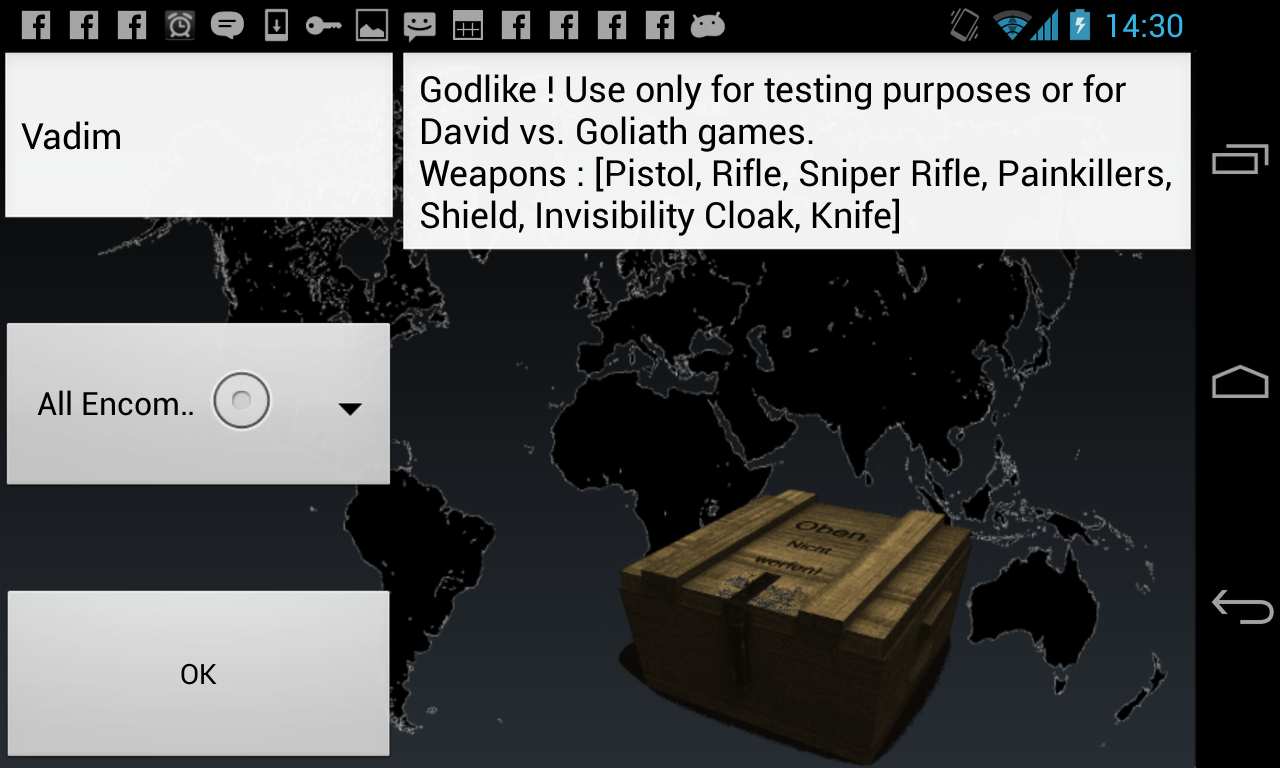
\includegraphics[height=3.5in,width=6.23in]{./images/android_screenshots/second_development/game_second_development_8.png}
  \caption{\small \sl Lobby settings screen with black background
  \label{fig:lobby_settings_background_black}}
  \end{figure}

  \begin{figure}
  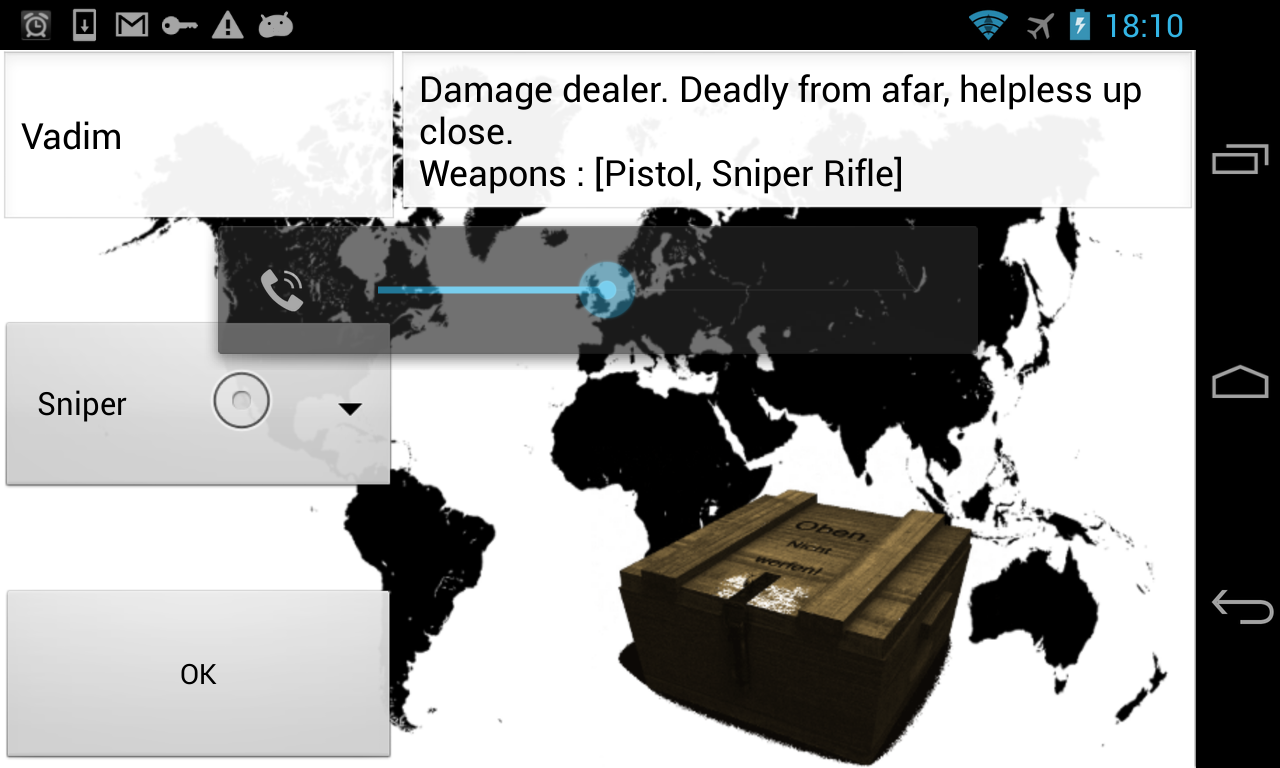
\includegraphics[height=3.5in,width=6.23in]{./images/android_screenshots/lobby_settings_background_white.png}
  \caption{\small \sl Lobby settings screen with white background
  \label{fig:lobby_settings_background_white}}
  \end{figure}
  
\end{enumerate}

\subsection{The second testing phase}

As the first testing phase, the second one has taken much less time than
initially planned - only one day. A larger number testers were invited. More
phones have been brought and almost all had 3G connections. This time, the app
supported Android versions starting with 2.3 - which made testing accessible to
all.\newline

A large part of the testing phase has consisted in the preparations: installing
the application on all devices, connecting everyone to the wireless network.
This has proven to be frustrating - therefore, everybody switched to 3G and
started to play - firstly indoors and soon after, outdoor. The UI changes have
been positively appreciated by everyone - yet a few features have proven to be
quite useless: One of them was the long click on the weapon buttons, which was
never used - because of close range gameplay, nobody attempted to draw the
weapon range. The gameplay has been very fast paced (a game lasted on average
between 10-15 minutes) and no one has actually used the functionality. The
distance indicator was not noticed at all by most testers. The health indicator,
target selection buttons and shooting functionality of the weapon buttons have
been appreciated as 'right', 'appropriate', 'useful'. A request was made for a
finishing condition and a 'You have won' screen for the winning team - and a
reward system. Because of the close-quarter gameplay, the starting condition
could not be tested - actually, a short workaround to disable it had to be
done.\newline

Unlike before the first testing phase, when few to no people interacted with
the application, before the second testing phase a large number of the friends
and acquaintances of the author have seen the application and have been giving
constant input as to whether certain aspects of the game are worthwhile or not.
Also at this point discussions on future development of the game have started. A
lot of conversations have been recorded as audio files and notes on paper. Among
the discussions, the ones on the current development have been focused on visual
aspects: The background images, the logo; a proposal to change all the markers
with 'profession'-specific ones and to replace the text on the buttons with
symbols. Besides all this, a discussion has started on the name of the
application itself. Both very positive and very negative opinions have been
expressed, but none of indifference. The first name chosen by the author for the
game has been ''People With Guns'' - but after debate and player feedback it has
been later changed to ''Gun Run''.\newline

There were ten people who actively participated in the discussions and debates
over the aforementioned aspects of the game: five male and five female.\newline

The logo has been strongly rejected by everybody - it was deemed too colourful
and unrelated to the significance of the game.\newline

The black background images used in the lobby and lobby settings screens have
been positively appreciated by the males but received mixed opinions from the
females: Three(more than half) of them said that the black backgrounds with
red weapons on top inspire violence - which should not represent the game, while
the other two have deemed them appropriate.\newline

After being presented with the white background images for the lobby and lobby
settings screens, everybody has rejected them, unanimously stating that they
break the atmosphere of the game. Everybody concluded that they prefer darker
colors in the menus.\newline

The second testing phase took a bit longer than the first. More players tried it
out, more games have been played and - most importantly - more games have been
played outside.\newline

The conclusion of the second test phase has been that the tutorials are too
long, too descriptive. The menus haven't received any criticism - but the game
UI has, in a passive manner: The long click functionality to draw the ranges of
the weapons has not been used at all. The distance indicator was not even seen
by the players and was therefore not used in any way by anyone. The
'Invisibility Cloak' powerup was used only by the current player on self, but in
the second stage of implementation it required selecting oneself(deselecting
everyone else) - this was deemed frustrating. The entire concept of selecting
oneself by deselecting all others(tapping an area on the map where no markers
are present) was deemed frustrating. Everybody playing has expressed the
necessity of symbols instead of text on the buttons and on the map. Another
aspect of criticism has been the order of the 'weapon'/'powerup' buttons: they
should be separated into two groups: 'weapons' and 'powerups'.\newline
